%%%%%%%%%%%%%%%%%%%%%%%%%%%%%%%%%%%%%%%%%%%%%%%%%%%%%%%%%%%%%%%%%%%%%%%%%%%%%%%%
% Template for USENIX papers.
%
% History:
%
% - TEMPLATE for Usenix papers, specifically to meet requirements of
%   USENIX '05. originally a template for producing IEEE-format
%   articles using LaTeX. written by Matthew Ward, CS Department,
%   Worcester Polytechnic Institute. adapted by David Beazley for his
%   excellent SWIG paper in Proceedings, Tcl 96. turned into a
%   smartass generic template by De Clarke, with thanks to both the
%   above pioneers. Use at your own risk. Complaints to /dev/null.
%   Make it two column with no page numbering, default is 10 point.
%
% - Munged by Fred Douglis <douglis@research.att.com> 10/97 to
%   separate the .sty file from the LaTeX source template, so that
%   people can more easily include the .sty file into an existing
%   document. Also changed to more closely follow the style guidelines
%   as represented by the Word sample file.
%
% - Note that since 2010, USENIX does not require endnotes. If you
%   want foot of page notes, don't include the endnotes package in the
%   usepackage command, below.
% - This version uses the latex2e styles, not the very ancient 2.09
%   stuff.
%
% - Updated July 2018: Text block size changed from 6.5" to 7"
%
% - Updated Dec 2018 for ATC'19:
%
%   * Revised text to pass HotCRP's auto-formatting check, with
%     hotcrp.settings.submission_form.body_font_size=10pt, and
%     hotcrp.settings.submission_form.line_height=12pt
%
%   * Switched from \endnote-s to \footnote-s to match Usenix's policy.
%
%   * \section* => \begin{abstract} ... \end{abstract}
%
%   * Make template self-contained in terms of bibtex entires, to allow
%     this file to be compiled. (And changing refs style to 'plain'.)
%
%   * Make template self-contained in terms of figures, to
%     allow this file to be compiled. 
%
%   * Added packages for hyperref, embedding fonts, and improving
%     appearance.
%   
%   * Removed outdated text.
%
%%%%%%%%%%%%%%%%%%%%%%%%%%%%%%%%%%%%%%%%%%%%%%%%%%%%%%%%%%%%%%%%%%%%%%%%%%%%%%%%

\documentclass[letterpaper,twocolumn,10pt]{article}
\usepackage{usenix2019_v3}

% to be able to draw some self-contained figs
\usepackage{tikz}
\usepackage{amsmath}
\usepackage{booktabs}
\usepackage{enumitem}
\usepackage{multirow}
\usepackage{pgfplots}
\usepackage{xcolor}
\usepackage{url}
\usepackage{subfigure}

% inlined bib file
\usepackage{filecontents}

%-------------------------------------------------------------------------------
\begin{filecontents}{\jobname.bib}
%-------------------------------------------------------------------------------
@Book{arpachiDusseau18:osbook,
  author =       {Arpaci-Dusseau, Remzi H. and Arpaci-Dusseau Andrea C.},
  title =        {Operating Systems: Three Easy Pieces},
  publisher =    {Arpaci-Dusseau Books, LLC},
  year =         2015,
  edition =      {1.00},
  note =         {\url{http://pages.cs.wisc.edu/~remzi/OSTEP/}}
}
@InProceedings{waldspurger02,
  author =       {Waldspurger, Carl A.},
  title =        {Memory resource management in {VMware ESX} server},
  booktitle =    {USENIX Symposium on Operating System Design and
                  Implementation (OSDI)},
  year =         2002,
  pages =        {181--194},
  note =         {\url{https://www.usenix.org/legacy/event/osdi02/tech/waldspurger/waldspurger.pdf}}}
\end{filecontents}

%-------------------------------------------------------------------------------
\begin{document}
%-------------------------------------------------------------------------------

%don't want date printed
\date{}

% make title bold and 14 pt font (Latex default is non-bold, 16 pt)
\title{\Large \bf TIC: A Tensor-Intact Compiling Infrastructure \\for Machine Learning Computers}

%%for single author (just remove % characters)
%\author{
%{\rm Your N.\ Here}\\
%Your Institution
%\and
%{\rm Second Name}\\
%Second Institution
%% copy the following lines to add more authors
%% \and
%% {\rm Name}\\
%%Name Institution
%} % end author

\maketitle

%-------------------------------------------------------------------------------
\begin{abstract}
%-------------------------------------------------------------------------------
Computers equipped with machine learning (ML) accelerators for improved efficiency have attracted increasing attentions recently. To effectively take advantage of ML computers, there is a huge demand for programming infrastructures to gain extremely high \emph{performance} across highly diverse ML architectures. Although existing programming tools are aware of the importance of the \emph{tensor} for easing the programming burden (e.g., TensorFlow and TVM), they still fail to well address this challenge. The main reason is that the high-level tensor semantic is broken during the lowering process with loss of tensor-level optimizations.

To address this problem, we propose the Tensor-Intact Compiling (TIC) infrastructure for improving the performance across different ML accelerators. The key intuition is that the \emph{tensor semantic can be well preserved thoroughly during the entire compilation process for ML accelerators}. The tensor semantic is primarily supported by the proposed Tensor Intermediate Representation (TIR) with multiple common tensor-level optimizations on the Tensor Abstract Machine (TAM). TAM is the foundation of TIC by abstracting the characteristics of tensor processing in a broad range of ML accelerators. Thus, tensor-level optimizations are general and can work well for various ML accelerators. In addition to treating traditional graph IR as the input, TIC also includes a domain-specific language, i.e., Tensor-Aware Language (TAL), for manually optimizing ML applications. Experimental results show that TIC outperforms state-of-art programming infrastructures on three commodity ML computers including GPU with Tensor Cores, TPU, and MLU.




%TIC consists of three main components: Tensor Abstract Machine (TAM), Tensor Intermediate Representation (TIR), and Tensor-Aware Language (TAL). TAM is the foundation of TIC by abstracting the characteristics of tensor processing in a broad range of ML accelerators for portability. TIR leverages the tensor primitives and memory hierarchy of TAM for automatically performing general optimizations with improved performance and productivity. TAL is a domain-specific language with tensor semantic for manually optimizing ML applications. Experimental results show that TIC significantly outperforms state-of-art programming infrastructures in terms of performance, productivity, and portability on three commodity ML computers including Tensor Core GPU, TPU and MLU.

%Computers equipped with machine learning (ML) accelerators for improved efficiency have attracted increasing attentions recently. To effectively take advantage of ML computers, there is a huge demand for programming infrastructures to gain extremely high \emph{performance}, to improve software \emph{productivity}, and to guarantee \emph{portability} across highly diverse ML architectures. Although existing programming tools are aware of the importance of the \emph{tensor} for easing the programming burden (e.g., TensorFlow and TVM), they still fail to well address all the above challenges. The main reason is that the high-level tensor semantic is broken during the lowering process with loss of potential optimizations.

%In this paper, we propose the Tensor-Intact Compiling (TIC) infrastructure for improving the performance, productivity, and portability. The key intuition is that the \emph{tensor semantic can be well preserved thoroughly during the entire compilation process for ML accelerators}. TIC consists of three main components: Tensor Abstract Machine (TAM), Tensor Intermediate Representation (TIR), and Tensor-Aware Language (TAL). TAM is the foundation of TIC by abstracting the characteristics of tensor processing in a broad range of ML accelerators for portability. TIR leverages the tensor primitives and memory hierarchy of TAM for automatically performing general optimizations with improved performance and productivity. TAL is a domain-specific language with tensor semantic for manually optimizing ML applications. Experimental results show that TIC significantly outperforms state-of-art programming infrastructures in terms of performance, productivity, and portability on three commodity ML computers including Tensor Core GPU, TPU and MLU.
\end{abstract}


%-------------------------------------------------------------------------------
\section{Introduction}
%-------------------------------------------------------------------------------

Machine learning (ML) algorithms have been widely used in a broad range of application fields, such as computer vision~\cite{liu2016ssd}, speech signal processing~\cite{amodei2016deep}, machine translation~\cite{bahdanau2014neural}, and robotics~\cite{redmon2015real}. To improve the processing efficiency of ML algorithms, heterogeneous computers with specialized ML accelerators have emerged to deliver significantly better performance and energy efficiency than general-purpose architectures. Typical commodity ML computers include NVIDIA's GPU with Tensor Cores specially designed for accelerating matrix and convolutional operations~\cite{markidis2018nvidia}, Google's Tensor Processing Units (TPU) for tensor operations~\cite{jouppi2017datacenter}, and Cambricon's Machine Learning Unit (MLU) for general machine learning operations~\cite{cambrion2016url}.


The programming infrastructure is crucial to effectively take advantage of various ML computers. However, the key challenge is to achieve high performance across highly diverse ML architectures. Figure~\ref{fig:challenge} shows that $4$ well-known programming infrastructures (i.e., TensorFlow~\cite{abadi2016tensorflow}, PyTorch~\cite{paszke2017automatic}, TVM~\cite{chen2018tvm}, and MLIR~\cite{Lattner2020MLIR}) perform significantly different on not only the same GPU platform but also four different platforms (i.e., CPU, GPU, Tensor Cores, and TPU), and no one can dominate the others. This challenge is mainly caused by non-trivial exploitation of highly parallel computation units and intricate memory hierarchy of ML hardware. Though ML compilers (e.g., XLA~\cite{tensorflow2016xla} and TVM) have emerged as a promising technique for automatically generating optimized code for different backend platforms, it still requires a great amount of expert efforts for achieving high performance, especially when porting to a new ML architecture. For example, TVM requires the programmers manually implementing dedicated schedules with tensorize primitives (e.g., split, fuse, and reorder), and the manual implemented schedules significantly vary for different ML architectures. 


%To take advantage of ML computers with minimal programming burden, the programming infrastructure needs to address major challenges of execution \emph{performance}, development \emph{productivity}, and platform \emph{portability}, which mainly stem from the dramatic diversity of $M$ applications and $N$ hardwares, as illustrated in Figure~\ref{fig:challenges}(a). The performance challenge is caused by non-trivial exploitation of highly parallel computation and intricate memory hierarchy of ML hardwares. Figure~\ref{fig:challenges}(b) shows that $4$ well-known programming infrastructures (i.e., TensorFlow~\cite{abadi2016tensorflow}, PyTorch~\cite{paszke2017automatic}, TVM~\cite{chen2018tvm}, and MLIR~\cite{Lattner2020MLIR}) perform significantly different on the same GPU platform. The productivity challenge for rapid development of applications on a specific ML architecture requires high-level abstraction and modularized programming interfaces. Figure~\ref{fig:challenges}(c) shows that the programming efforts in terms of LoCs (Lines of Code) of evaluated programming infrastructures are quite different on the same GPU platform. The portability challenge inevitablly exists between different architectures as highly optimized code is hard to be migrated to others. Figure~\ref{fig:challenges}(d) shows that the performance portability\footnote{A quantitative metric introduced in \cite{pennycook2019implications} to evaluate performance portability for a given application across different platforms.} of a given application (i.e., ResNet-50) is dramatically different across $4$ hardware platforms. Such relatively controdictory challenges call out for dedicated programming infrastructures to bridge the gap between various ML applications and architectures.

%which is demonstrated by significantly different LoCs for $5$ applications in Figure~\ref{fig:challenges}(c). The (performance) portability challenge inevitably exists between different architectures as highly optimized code is hard to be migrated to others (e.g., AVX is only available on Intel's platforms), and the same application performs dramatically different across $4$ platforms in Figure~\ref{fig:challenges}(d). Such relatively contradictory challenges call out for dedicated programming infrastructures to bridge the gap between ML applications and architectures.

\begin{figure}[t]
%\vspace{-5pt}
\centering
  \subfigure[GPU platform]{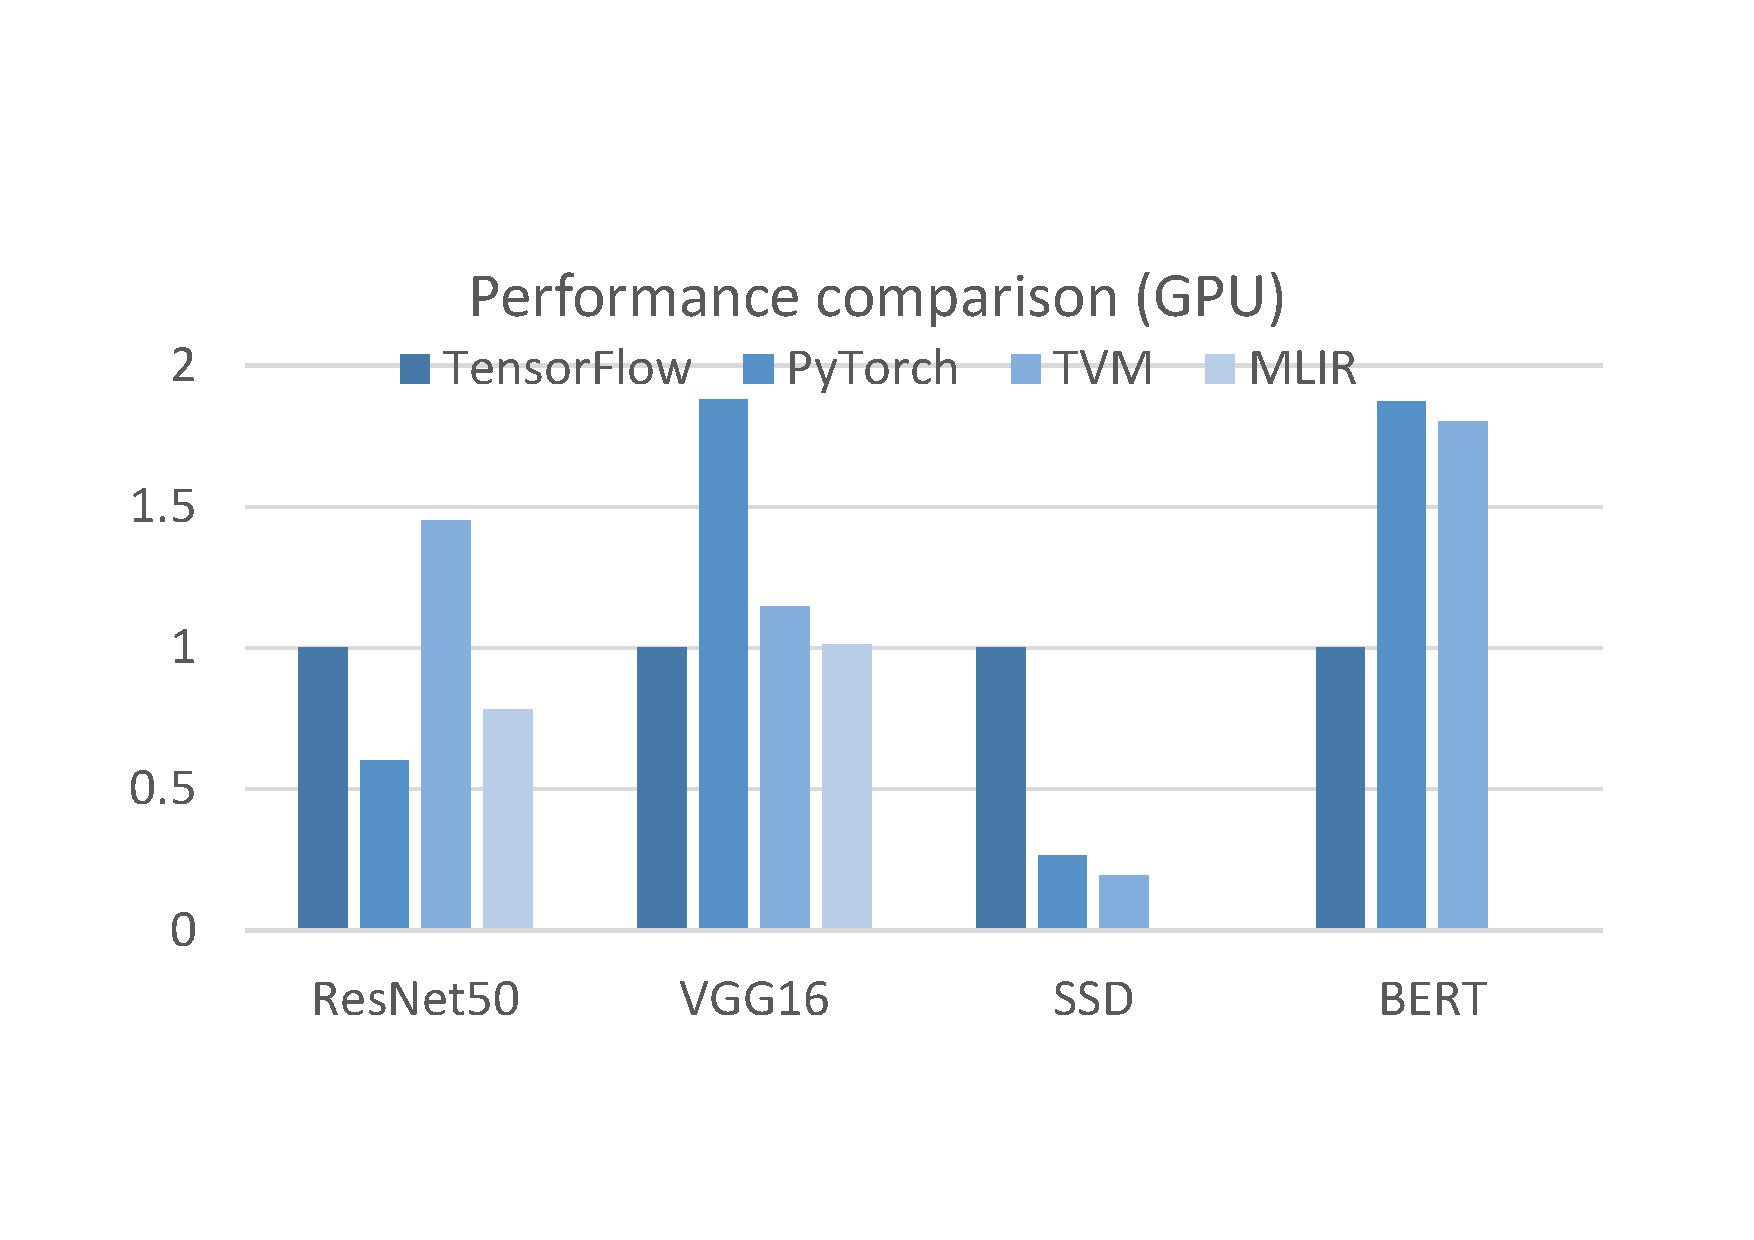
\includegraphics[width=0.49\columnwidth]{figures/intro-perf-gpu.pdf}}
  \subfigure[Cross-platform]{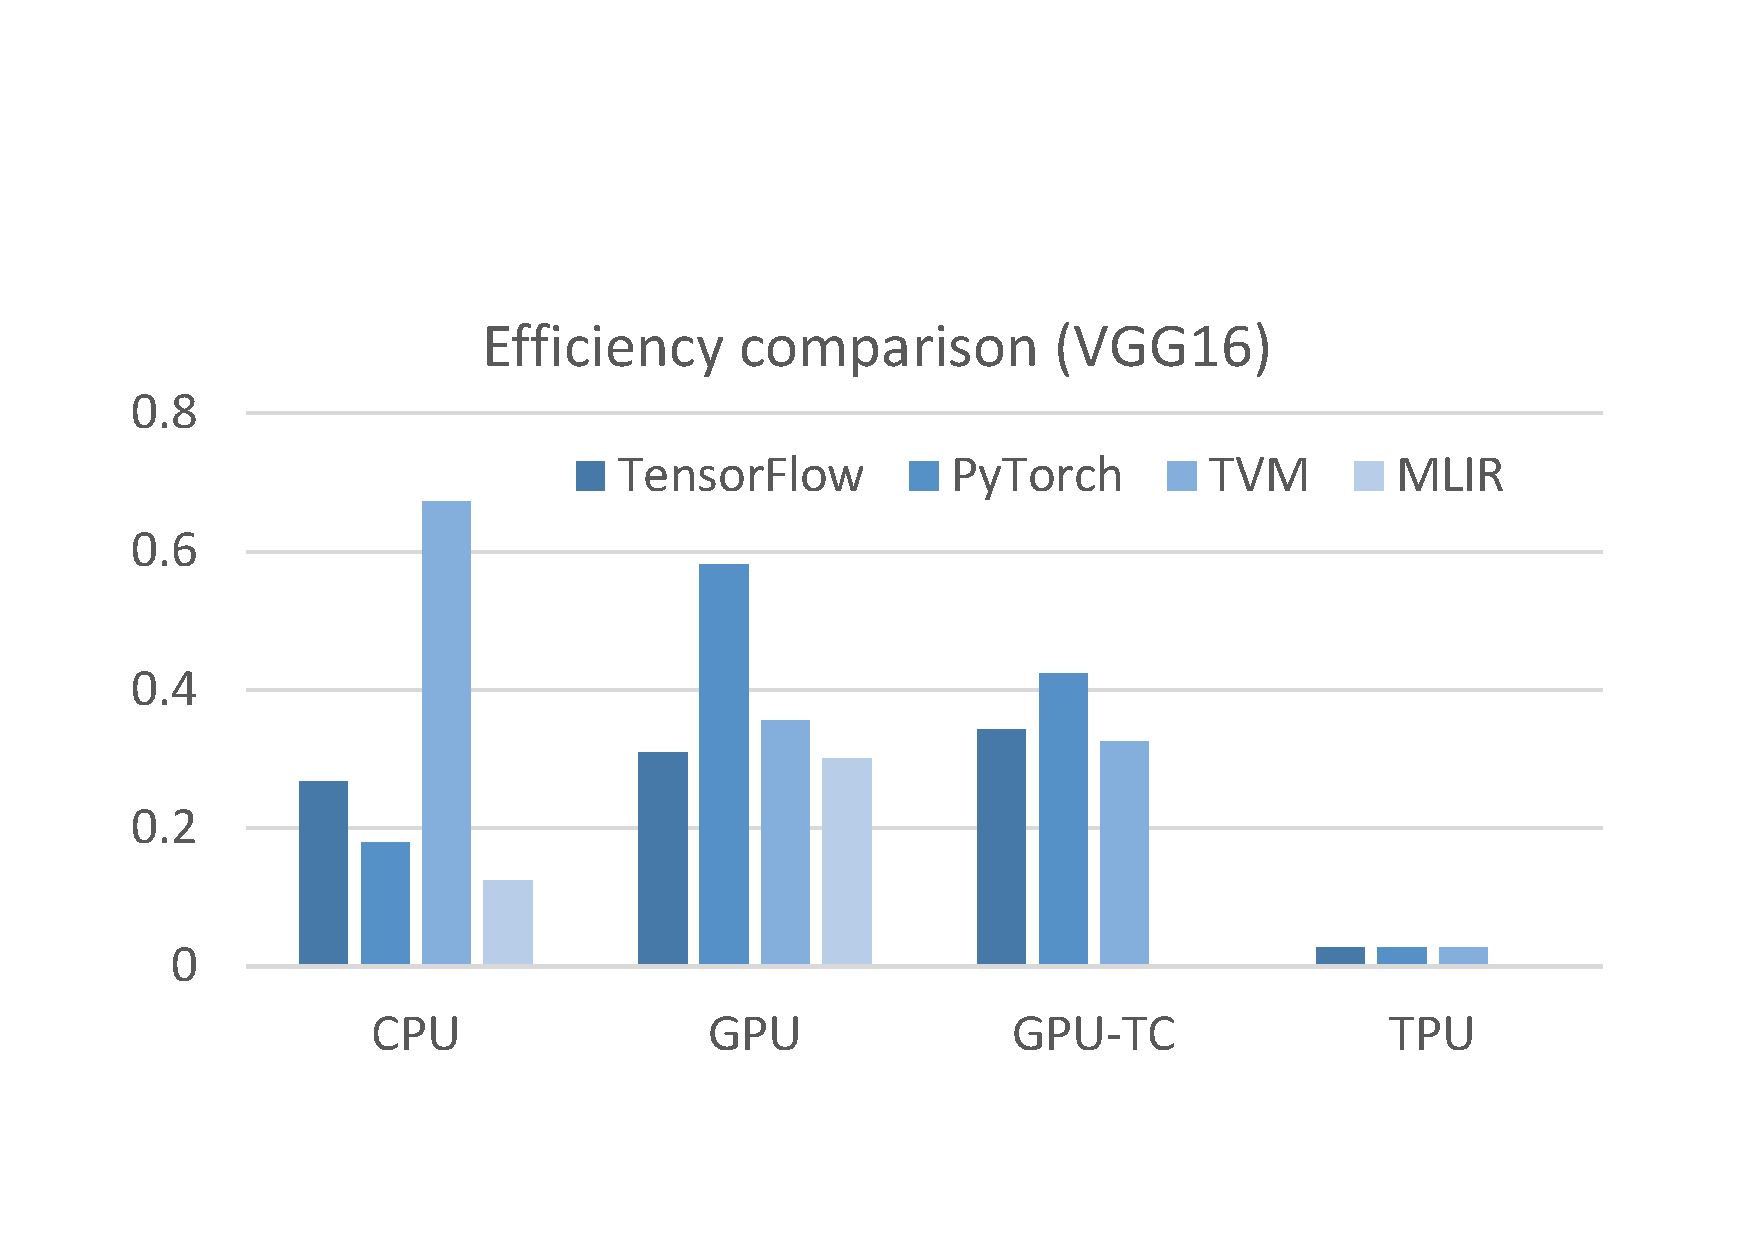
\includegraphics[width=0.49\columnwidth]{figures/intro-eff.pdf}}
  \vspace{-8pt}
\caption{\footnotesize The comparison of four programming infrastructures (i.e., TensorFlow, PyTorch, TVM, and MLIR). (a) It is hard to optimize the performance of applications for different programming infrastructures even on the same GPU platform (the performance is normalized to that of TensorFlow). (b) Even for the same application (VGG16~\cite{simonyan2014very}), the efficiency (i.e., hardware utilization) varies significantly across different platforms for evaluated programming infrastructures. Apparently, none of the above programming infrastructures can dominate others for exploiting the computational ability.}
%The key challenges of programming infrastructures for ML computers, which are mainly caused by the huge gap between $M$ ML applications and $N$ hardwares. (b) The \emph{performance} challenge: it is hard to optimize the performance of applications with $4$ different programming infrastructures (i.e., TensorFlow, PyTorch, TVM, and MLIR) even on the same GPU platform (the higher the better). (c) The \emph{productivity} challenge: the programming efforts of applications vary significantly for different infrastructures even on the same GPU platform (the lower the better). (d) The \emph{portability} challenge: for a specific application (i.e., ResNet50), the performance portability is different across $N$ platforms (the higher the better). Apparently, none of the above programming infrastructure can dominate others.}
%given a specific application, it is hard to optimize the performance even on one platform ($1$ vs $1$). (c) The productivity challenge: given $M$ applications, the productivity varies significantly even on one platform ($M$ vs $1$). (d) The portability challenge: given a specific application, it is hard to ensure performance portability across different platforms ($1$ vs $N$).}
\label{fig:challenge}
\vspace{-5pt}
\end{figure}

%Currently, there are four main progamming infrastructures for ML computers, i.e., programming frameworks, languages, libraries, and ML compilers. The programming frameworks (e.g., TensorFlow and PyTorch) offer great productivity with the help of high-level languages and APIs but notoriously low efficiency. For example, running PyTorch on V100 GPU only achieves 9\% of the peak performance for ResNet-50. The programming languages (e.g., CUDA) provide flexibility and programmability for easily adapting to new ML algorithms at the cost of productivity and portability, epsecially for achieving performance portability across different platforms. The programming libraries (e.g., CUDNN~\cite{chetlur2014cudnn}) can deliver high performance at the cost of low portability. For example, even with well-defined and widely-used BLAS (Basic Linear Algebra Subroutines) inferface~\cite{blas}, the programming libraries cannot be migrated across different platforms such as GPU and TPU. Recently, ML compilers (e.g., XLA~\cite{tensorflow2016xla} and TVM) have emerged as a promising technique for addressing performance, productivity, and portability challenges. However, whether such challenges are well addressed by existing ML compilers remains an open question.%, especially for highly diverse ML hardwares with continuously evolving ML algorithms.

The key reason of the inefficiency of existing programming infrastructures (including ML compilers) is that \emph{the critical tensor semantic generated from the high-level programming interfaces is broken during the lowering process for ML accelerators, which directly process tensor semantic as well}. Here we use two motivating examples in TensorFlow and TVM to demonstrate that breaking the tensor semantic during compilation is inefficiency for ML architectures.


%though most of them directly handle tensors instead of scalars, e.g., TensorFlow characterizes the execution as dataflow graphs by carrying \emph{tensors} on the edges. Here we use two motivating examples in TensorFlow and TVM to demonstrate that breaking the tensor semantic during compilation is inefficiency for ML architectures.

\textbf{Framework example (e.g., TensorFlow).} Figure~\ref{fig:intro-tf} shows the overall execution of the \texttt{max\_pool} operation in TensorFlow, where the tensor semantic is broken during the implementation of this operation, i.e., from the high-level TensorFlow API to the low-level CUDA implementation. In the CUDA code, the original \texttt{max\_pool} operation is broken into scalar operations (e.g., conditional comparison) with multiple loops. Thus, for the ML architecture equipped with tensor instructions (e.g., \texttt{VGTM}, Vector-Greater-Than-Merge instruction in~\cite{liu2016cambricon,chen2019instruction}), non-trivial optimization (e.g., notorious auto-parallelization) should be conducted either manually or automatically on the scalar operations to leverage such tensor instructions, which is extremely hard and may result in low performance and huge efforts.

%A potential solution is to extend the low-level language to directly support tensor instructions.

\begin{figure}[t]
  \centering
%  \vspace{-5pt}
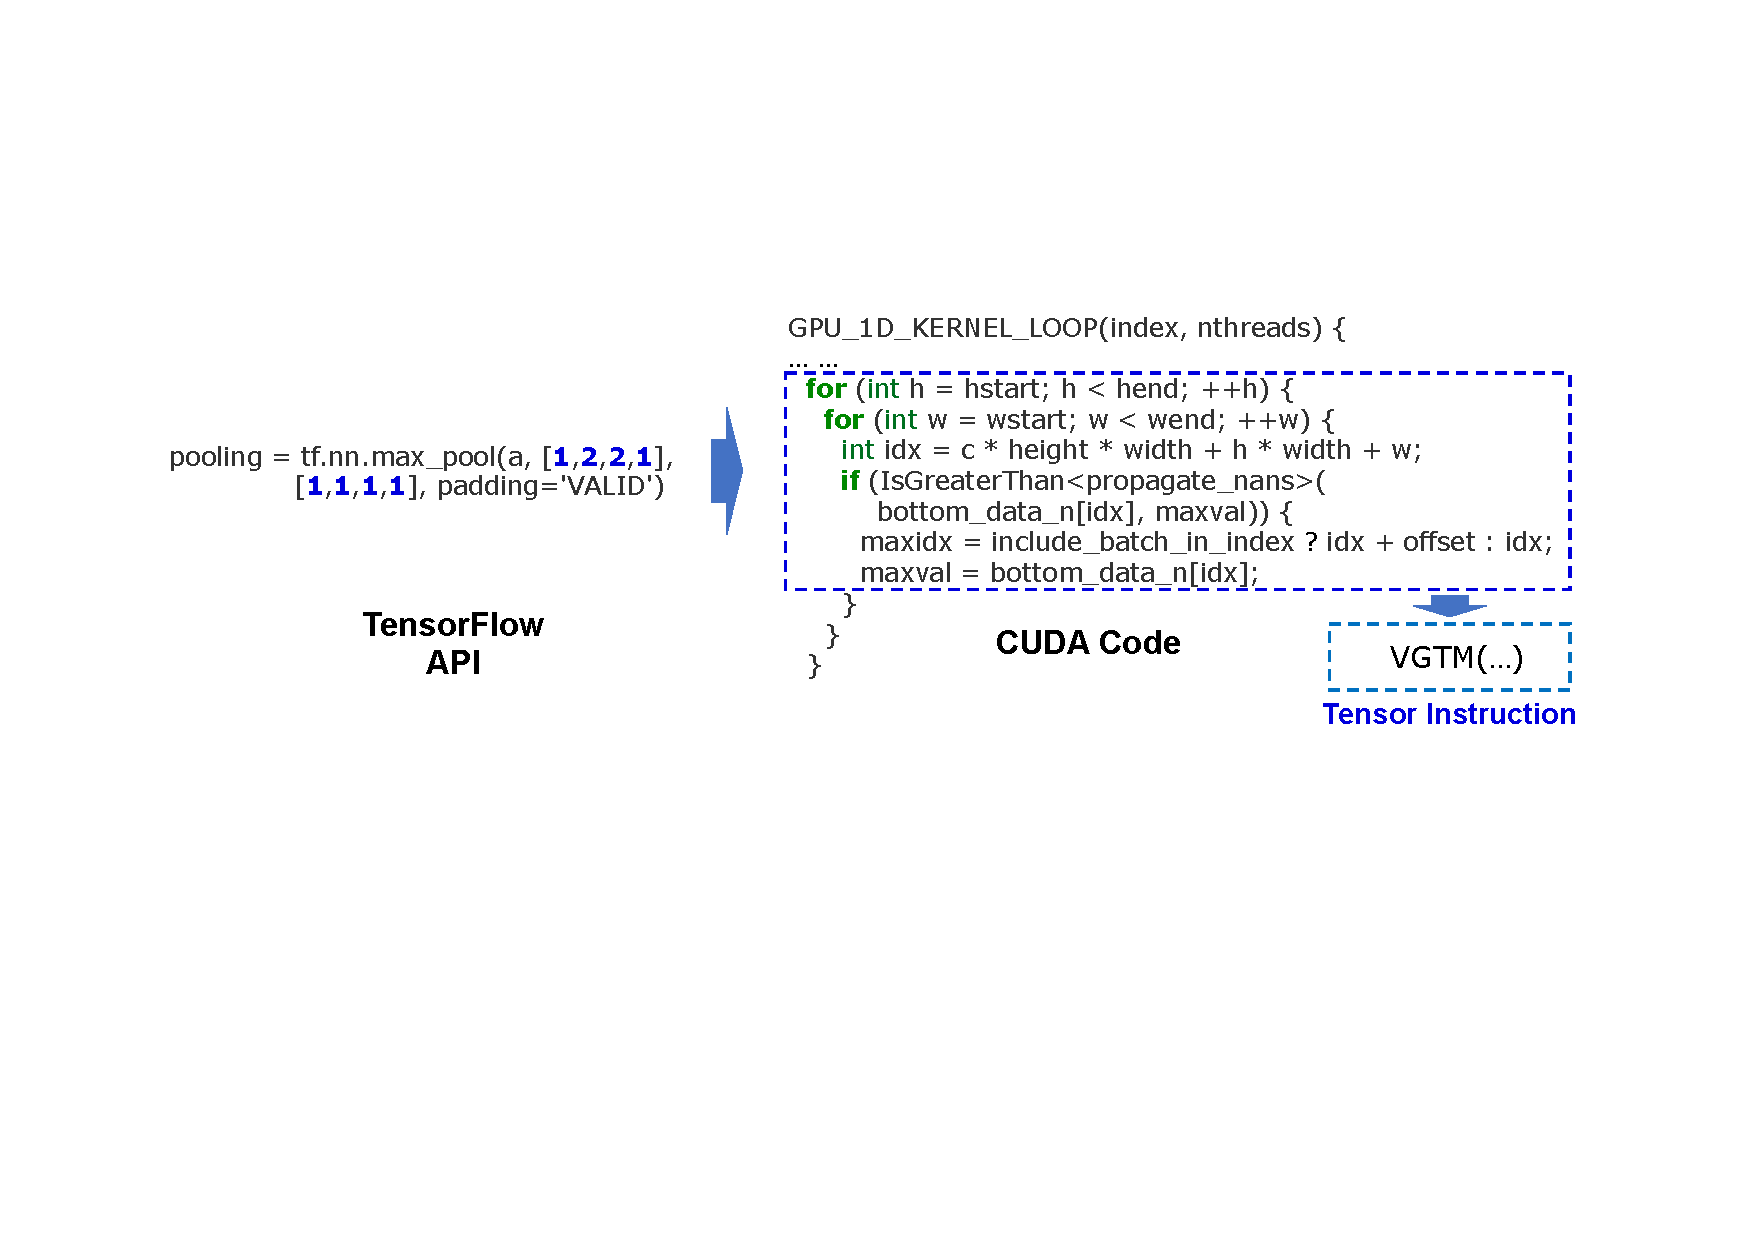
\includegraphics[width=1.0\columnwidth]{figures/intro-tf.pdf}
\vspace{-15pt}
\caption{\footnotesize The tensor semantic is broken from the high-level \emph{tensor} API to low-level \emph{scalar} implementation, which makes it extremely hard to exploit the tesnor instructions (e.g., \texttt{VGTM}) of ML hardware from the low-level code.}
\label{fig:intro-tf}
\vspace{-15pt}
\end{figure}

\textbf{ML compiler example (e.g., TVM).} Figure~\ref{fig:intro-tvm} shows the execution of the \texttt{conv} operation in TVM for GPU with Tensor Cores (GPU-TC) and Cambricon-ACC (CACC)~\cite{chen2019instruction}, where the input is Relay's graph IR that directly processes tensors. After converting the Relay IR to the TVM IR, the tensor operation is lowered into multiple loops with scalar multiply and add operations. Then, the TVM IR can be \emph{tensorized} to target platforms with tensor-related primitives, such as \texttt{wmma::mma\_sync} and \texttt{conv} in GPU-TC and CACC, respectively. Apparently, such ``tensor-scalar-tensor" process is relatively tedious and error-prone for either manually or automatically leveraging tensor-related primitives and inflexible for enforcing tensor-level optimizations such as tensor decomposition and tensor pipeline. In addition to low productivity and potential performance loss, the optimization on TVM IR for supporting tensor primitives is not portable across different architectures. For example, \texttt{wmma::mma\_sync} cannot be executed on CACC. %Therefore, it is necessary to provide abstraction of common tensor processing of underlying ML architectures to improve the portability.

\begin{figure*}
\centering
%\vspace{-10pt}
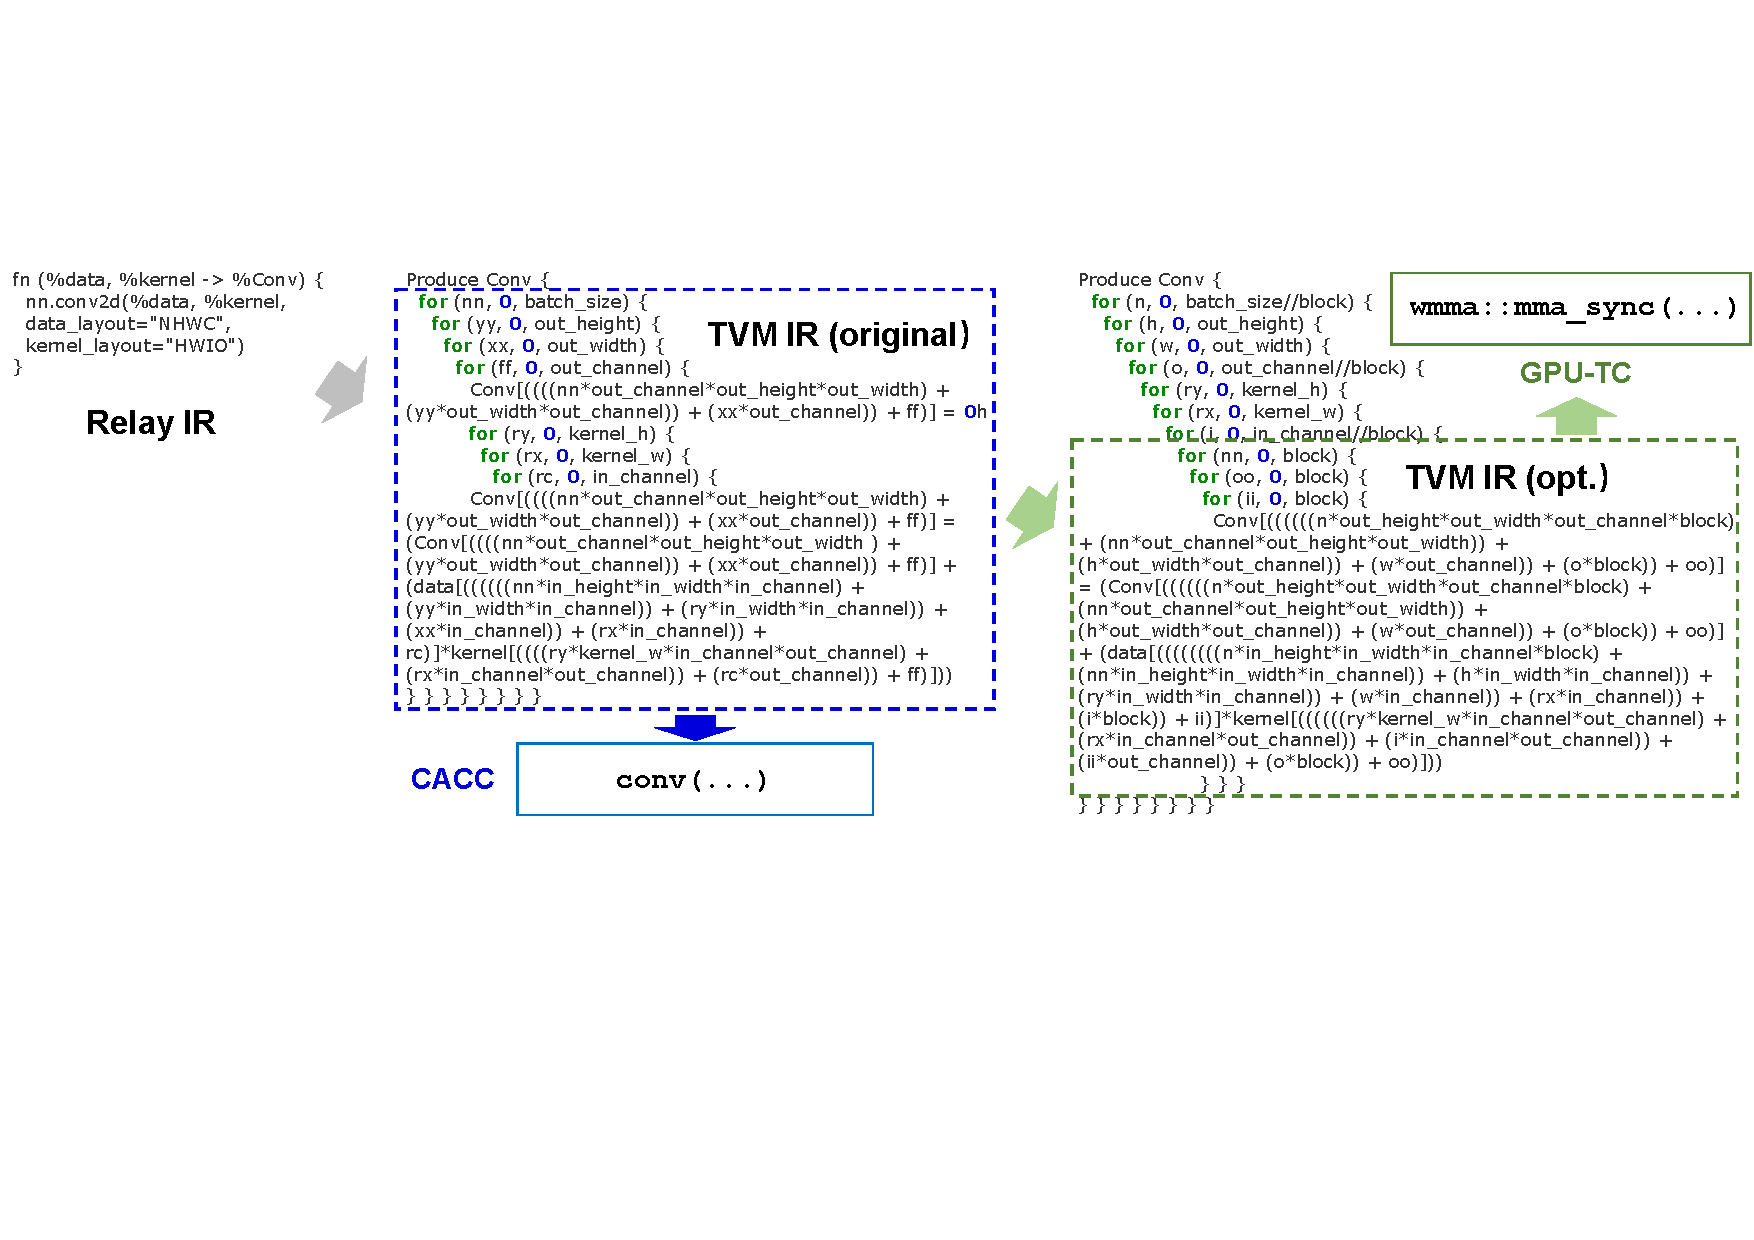
\includegraphics[width=0.9\textwidth]{figures/intro-tvm.pdf}
\vspace{-5pt}
\caption{\footnotesize The tensor semantic is broken during the lowering process in TVM for GPU with Tensor Cores (GPU-TC) and Cambricon-ACC (CACC), where the ``tensor-scalar-tensor" process is relatively tedious and may lose potential performance optimization, For GPU-TC, the original IR requires dedicated optimization for using \texttt{wmma:mma\_sync}. For CACC, it is relatively intuitive for using the \texttt{conv} primitive. Also, the direct extension of TVM IR for supporting tensor primitives without abstraction of various ML architectures results in low portability across different platforms.}
\label{fig:intro-tvm}
\vspace{-5pt}
\end{figure*}

\textbf{Our solution.} Based on the above observation, in this paper, we propose the Tensor-Intact Compiling (TIC) infrastructure for ML computers. As shown in Figure~\ref{fig:intro-comp}, the key of TIC is to replace the previous scalar-based low-level IR with tensor-based IR (i.e., Tensor Intermediate Representation, TIR), which can represent tensor primitives and specific memory hierarchy for tensor processing, so that the tensor semantic can be preserved from the input high-level IR (e.g., Relay IR, TensorFlow Graph IR) to tensor-oriented hardware platforms (e.g., GPU-TC, TPU, and CACC). In order to perform tensor-related optimizations, an abstract tensor machine (i.e., Tensor Abstract Machine, TAM) is proposed for concealing the huge variety of ML architectures. Specifically, by raising the level of abstraction of tensor processing in various ML architectures, many common hardware-aware optimizations such as \emph{tensor decomposition} and \emph{tensor alignment} can be conducted at high levels to alleviate the porting burden across different platforms. This is completely different in previous approaches where the tedious manual or semi-automatic tensorization should be performed for each platform. Moreover, in addition to high-level tensor-based IR, we also propose a domain-specific language, Tensor-Aware Language (TAL), with tensor semantic and hardware characteristics (e.g., memory hierarchy and control logic) for manually achieving extremely high performance. To our best knowledge, such a compiling infrastructure preserving tensor sematic across abstract hardware machine, hardware-aware IR, and programming language is the first holistic solution for addressing the performance challenge of various ML computers.

%There are two intuitions for building such a tensor-aware compiling infrastructure. The first is that all the stated challenges are somewhat controdictory to each other, and a single component at a specific layer cannot well address all these challenges. The second is that by preserving tensor semantic during compilation in a holistic manner can easily bring more optimization opportunities. As a result, by constructing the tensor-intact compiling infrastructure from a hardware/software vertical perspective, TIC consists of three components, i.e., Tensor Abstract Machine (TAM), Tensor Intermediate Representation (TIR), and Tensor-Aware Language (TAL). TAM is the basis of TIC and crucial to the performance portability since there is a huge variety of ML architectures. By raising the level of abstraction of tensor processing in various ML architectures, many common hardware-aware optimizations can be conducted at high levels to alleviate the porting burden across different platforms. TIR is a tensor IR that leverages the tensor primitives and memory hierarchy of TAM with improved performance and productivity. TAL is a domain-specific language with tensor semantic and hardware characteristics (e.g., memory hierarchy and control logic) for manually achieving extremely high performance. To our best knowledge, such a compiling infrastructure preserving tensor sematic across abstract hardware machine, hardware-aware IR, and programming language is the first holistic solution for addressing all stated challenges.

\begin{figure}[t]
  \centering
  \vspace{-5pt}
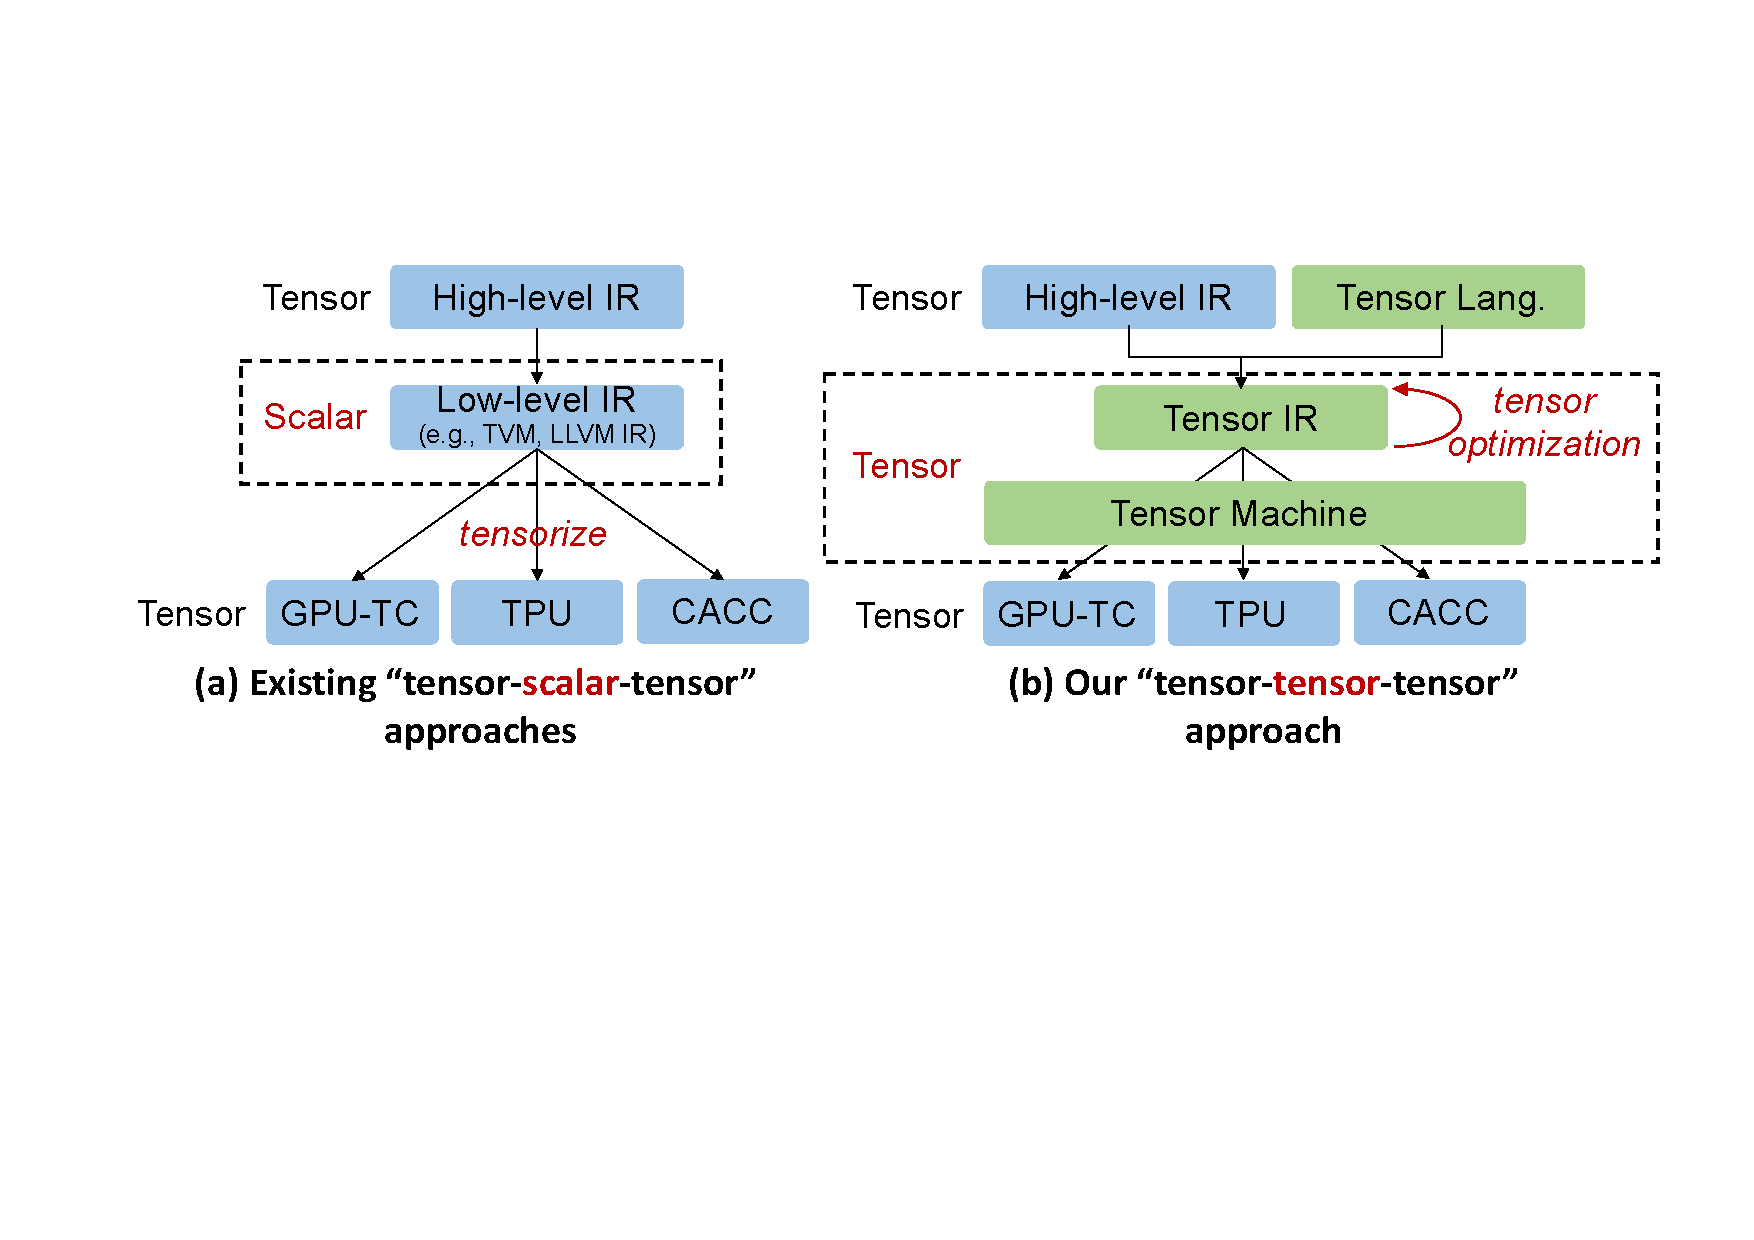
\includegraphics[width=1.0\columnwidth]{figures/intro-comp.pdf}
\vspace{-15pt}
\caption{\footnotesize Comparison between our solution and previous ``tensor-scalar-tensor" process.}
\label{fig:intro-comp}
\vspace{-10pt}
\end{figure}


%\textbf{Our solution.} Based on the above observation, in this paper, we propose the Tensor-Intact Compiling (TIC) infrastructure for ML computers. There are two intuitions for building such a tensor-aware compiling infrastructure. The first is that all the stated challenges are somewhat contradictory to each other, and a single component at a specific layer cannot well address all these challenges. The second is that by preserving tensor semantic during compilation in a holistic manner can easily bring more optimization opportunities. As a result, by constructing the tensor-intact compiling infrastructure from a hardware/software vertical perspective, TIC consists of three components, i.e., Tensor Abstract Machine (TAM), Tensor Intermediate Representation, and Tensor-Aware Language (TAL). TAM is the basis of TIC and crucial to the performance portability since there is a huge variety of ML architectures. By raising the level of abstraction of tensor processing in various ML architectures, many common hardware-aware optimizations can be conducted at high levels to alleviate the porting burden across different platforms. TIR is a tensor IR that leverages the tensor primitives and memory hierarchy of TAM with improved performance and productivity. TAL is a domain-specific language with tensor semantic and hardware characteristics (e.g., memory hierarchy and control logic) for manually achieving extremely high performance. To our best knowledge, such a compiling infrastructure preserving tensor sematic across abstract hardware machine, hardware-aware IR, and programming language is the first holistic solution for addressing all stated challenges.


To demonstrate the efficiency of our approach, we conduct extensive experiments with different applications on $3$ commodity ML computers, i.e., GPU-TC, TPU, and MLU. We compare TIC with different programming infrastructures: %(1) compared to PyTorch with vendor-provided libraries, the performance gains are XX, XX, and XX, on GPU-TC, TPU, and MLU, respectively;
(1) compared to TensorFlow, the performance gains are 12.2\%, 1.4\%, and 51.7\%, on GPU-TC, TPU, and MLU, respectively; (2) compared to the ML compiler XLA, the performance gains are 2.4\%, 1.5\%, and 34.6\% on GPU-TC, TPU, and MLU, respectively; and (3) compared to the ML compiler TVM, the performance gains are 12.8\%, 1.3\%, and 44.9\%, on GPU-TC, TPU, and MLU, respectively. In addition, the portability of TIC is also evaluated by using the performance portability~\cite{pennycook2019implications} when porting to different platforms. Experimental results show that compared to TensorFlow, XLA, and TVM, TIC improves the performance portability by 22\%, 10.9\%, and 28.4\%, respectively.%, and reduces the porting efforts in terms of LoCs by XX\%, XX\%, and XX\%, respectively,

%In terms of productivity, we compare the LoCs of different programming infrastructures for implementing both high-level networks and core operators on a specific platform (i.e., GPU-TC). Experimental results show that for implementing networks, TIC outperforms TensorFlow, TVM, MLIR by XX\%, XX\%, and XX\%, respectively, and for implementing core operators, TIC outperforms TensorFlow, TVM, MLIR by XX\%, XX\%, and XX\%, respectively. 

%and results show that the LoCs can be reduced by XX\% and XX\% on GPU-TC and MLU, respectively. Compared with other programming frameworks, the productivity remains as the high level inferaces (e.g., the APIs of frameworks) for users are preserved. %Also, we present a case study on using TIC for rapid development and optimization of an end-to-end application on a typical ML computer.



%\textbf{Contributions.} In contrast to existing ``scalar-to-tensor" tensorization approaches, this work first proposes ``tensor-to-tensor" decomposition approach, which makes the following contributions.
\textbf{Contributions.} This paper makes the following contributions:

\begin{itemize}
\vspace{-7pt}
\item \textbf{Abstract ML machine.} The abstract ML machine is built by extracting key and common features of tensor processing of various ML architectures. Thus, concrete ML platforms (e.g., GPU-TC and MLU) can benefit from the common hardware-aware optimizations at high levels, which can improve both the performance and portability, This is the first work on characterizing the common features for obtaining a unified programming model of diverse ML architectures.

\vspace{-7pt}
\item \textbf{Hybrid IR.} The hybrid IR describes both scalars and tensors, and the benefit is three-fold. The first is to integrate to existing frameworks and graph IRs to leverage their easy-to-use interfaces. The second is to alleviate implementation efforts for the developers of frameworks and libraries. The third is to exploit potential optimization opportunities on the tensors.

\vspace{-7pt}
\item \textbf{Tensor-aware language.} The tensor-aware language is a domain-specific language with tensor semantic and hardware characteristics. The language can be used for more flexibility and high performance.

\vspace{-7pt}
\item \textbf{Systematic evaluation.} We systematically evaluate the performance and portability of different programming infrastructures (TensorFlow, TVM, MLIR, and TIC) on various platforms (GPU-TC, TPU, and MLU), and experimental results well demonstrate the effectiveness and efficiency of TIC.


\end{itemize}


\section{Overview}\label{sec:overview}

\begin{figure}
\vspace{-10pt}
\centering
\includegraphics[width=0.85\columnwidth]{figures/overview.pdf}
\vspace{-10pt}
\caption{\footnotesize The entire programming stack integrated with the proposed Tensor-Intact Compiling (TIC) infrastructure.}
\label{fig:overview}
\vspace{-15pt}
\end{figure}

Figure~\ref{fig:overview} presents the entire programming stack integrated with the proposed TIC compiling infrastructure. For various ML applications, to provide sufficient productivity, the programming frameworks are used as the primary programming interfaces for building networks. The built networks will be converted to graph-level Intermediate Representation such as TensorFlow's Graph~\cite{abadi2016tensorflow} and Relay~\cite{roesch2018relay}, where various graph-level optimizations~\cite{tensorflow2016xla} can be performed. Such optimization passes may include constant folding, operation fusion, and graph substitution~\cite{jia2019taso}. The optimized graph will be treated as the input for the low-level hybrid IR, i.e., TIR, where both scalar and tensor-related optimization passes can be applied.  Since TIR is built upon TAM that extracts common hardware characteristics of various ML architectures, many common optimizations enforced on TIR take effects for different architectures, which significantly alleviates the optimization burden of backends. As the abstraction of various ML hardware, TAM incorporates abstracted tensor instructions that can be easily translated to platform-specific instructions such as \texttt{wmma} of GPU-TC and \texttt{conv} of Cambricon-ACC. In addition to using the graph IR as input, programmers can directly use TAL to not only implement the core operators (e.g., \texttt{conv} and \texttt{mlp}) in the frameworks but also the end-to-end applications. The original TAL programs will be translated to the TIR for further optimization as well.

\textbf{Programming example.} As stated, the TAM can be programmed either from the graph-level IR such as Relay or the domain-specific TAL. Here we use the Relay as the graph IR and it can take the models of various frameworks as inputs. Thus, legacy programs written with frameworks or Relay interfaces can be directly executed with TIC.


With TAL, a simple network consisting of one convolution operation can be implemented as follows, where the \texttt{pnm} and \texttt{pwm} are different types of on-chip memory, which will be detailed in Section~\ref{sec:mlam}. The \texttt{conv} function processes tensor inputs, which will be eventually mapped to the corresponding tensor instruction of TAM.

\vspace{-8pt}
\begin{scriptsize}
\begin{verbatim}
__pnm__ Tensor in(DT_FP16, Format("NHWC"), Shape({N, H, W, CI}));
__pnm__ Tensor out(DT_FP16, Format("NHWC"), Shape({N, H, W, CO}));
__pwm__ Tensor wgh(DT_FP16, Format("HWIO"), Shape({KH, KW, CI, CO}));
...
__conv(out, in, wgh, sx, sy);
...
\end{verbatim}
\end{scriptsize}
\vspace{-15pt}

\section{TAM: Tensor Abstract Machine}\label{sec:mlam}

\begin{figure}[t]
  \centering
%  \vspace{-10pt}
\includegraphics[width=0.95\columnwidth]{figures/TAM2instances.pdf}
\vspace{-10pt}
\caption{\footnotesize Tensor abstract machine (TAM) and its instances. \textbf{(a)} A 1-level
  TAM which serves as the basic block to build multi-level
  instances.\textbf{(b)} A 2-level TAM, which is able to describe
  current mainstream ML architectures. \textbf{(c)} TAM instance:
  Cambricon-ACC. \textbf{(d)} TAM instance: multi-cluster
  Cambricon-ACC (MCACC). \textbf{(e)} TAM instance: TPU. \textbf{(f)} TAM instance:
  GPU-TC.}
\label{fig:vm}
\vspace{-12pt}
\end{figure}


In this section, we introduce the tensor abstract machine (TAM) with virtual
instruction set architecture (vISA). To well model a broad range of ML architectures
in a general manner, TAM should be able to express the following major characteristics
commonly existed in current ML architectures, including the massive
functional units for data-level parallelism (e.g., thousands of MACs in
TPU~\cite{jouppi2017datacenter}), the memory hierarchy for leveraging data
locality in ML algorithms (e.g., global and shared memory in GPUs~\cite{ghorpade2012gpgpu}.),
and the tensor-level instructions for simple control (e.g., matrix/vector
instructions in Cambricon~\cite{liu2016cambricon}).


\subsection{TAM model}
In Figure~\ref{fig:vm} (a), we show the proposed TAM, which consists of three
major parts that are visible to programmers, i.e., the computation logic, the
memory, and the control logic.

\textbf{Computation logic.} The computation logic includes a
parallel functional unit (PFU) and a serial functional unit (SFU). The PFU is
able to perform tensor operations, including convolution, matrix multiplication,
and inner production. The PFU can have different design choices. For example,
TPU~\cite{jouppi2017datacenter}, ShiDianNao~\cite{du2015shidiannao}, and Eyeriss~\cite{chen2016eyeriss},
leverage systolic array architecture, which organizes multiple scalar
MACs in a 2-D mesh topology to perform tensor
operations. DianNao~\cite{chen2014diannao} leverages several vector operation units as hardware
neurons to perform tensor operations. The SFU usually performs scalar operations (e.g.,
ALU), which might be omitted in some ML architectures.

\textbf{Memory.} The memory part includes a parallel neuron memory (PNM)
and a parallel weight memory (PWM) for the PFU. Inline with the observation in~\cite{pudiannao} where
many machine learning techniques can separate memory
accesses into different data flows, TAM includes two separate on-chip memory
for the PFU. In order to flexibly support different memory access
patterns, TAM allows data transfer between off-chip and on-chip
memory, as well as data transfer between PNM and PWM. Note that since
both the PNM and the PWM are visible
to programmers (i.e., scratchpad memory), they are managed by programmers
explicitly; hardware cache is transparent to programmers, they cannot be seen in TAM.


\textbf{Control logic.}
In TAM, the abstracted controller is built to manage all the modules to
perform tensor-level operations. Roughly, it has three major functionalities in
its FSM states: DMA control, task status management, and pipeline execution
management. The DMA control allows the data exchange directly between on-chip
buffer and off-chip memory, including both program data and instruction
sequence. The task status management contains task load, start, execution,
stop, and stall, when performing ML tasks on TAM. The pipeline execution
management maps the instruction sequence to the computing units. 


Particularly, TAM adopts a tensor-level virtual ISA to support tensor
operations in ML. In
Table~\ref{tab:virtualISA}, we list representative instructions in vISA proposed for
TAM. The vISA consists of the scalar and tensor instructions,
and they both contains instructions for arithmetic, logic, and data
transfer. Besides, the scalar instructions contain several instructions for
control, i.e., \texttt{jump}, \texttt{branch}, \texttt{sync}; the tensor instructions
contain several instructions for function operations at higher levels, such as
\texttt{conv}, \texttt{pooling}, and \texttt{gemm}. Note that the
\texttt{sync} instruction is used for synchronizing the execution between the
scalar units and tensor units. 


\begin{table}[b]
  \centering
  \scriptsize
  \vspace{-25pt}
  \caption{\footnotesize Typical instructions of the proposed vISA.}
  \label{tab:virtualISA}
  \begin{tabular}{llllllllll}
    \toprule
    Type &&Instructions\\
    \midrule
    Scalar &arithmetic& \texttt{add, sub, mult, div} \\
    &logic&\texttt{eq, less, great}\\
    &control&\texttt{jump, branch, sync}\\
    &data&\texttt{load, store, move}\\
    \midrule
    Tensor&function&\texttt{conv, pooling, gemm}\\
    &arithmetic&\texttt{mult, add, sub, element-wise}\\
    &logic&\texttt{min, max}\\
    &data&\texttt{load, store, move}\\
    \bottomrule
  \end{tabular}
%  \vspace{-10pt}
  \end{table}



\textbf{Multi-level TAM.} TAM allows multi-level abstraction for accurately modeling a large number of existing
ML architectures. In Figure~\ref{fig:vm}(b), we show a 2-level TAM extended from
the basic 1-level TAM shown in Figure~\ref{fig:vm}(a). Roughly, the 2-level TAM
contains several 1-level TAMs with a shared memory (i.e., the parallel shared
memory, PSM) connected with each other. 
Note that the PSM can be either globally shared for all 1-level TAMs or partially shared by a group of them. 
Apparently, ML architectures with more levels can be modeled by multi-level TAM
in the same principle. In this paper, we focus on 2-level TAM as it is
able to model current mainstream ML architectures. 


\subsection{TAM instantiation}
To ease the burden of TAM instantiation, we define a in-house protocol
to describe a certain TAM instance from the TAM abstraction. The protocol can be
taken as a configuration of TAM with specific parameters (e.g., PSM size, PFU
organization) and more importantly, instruction mapping from virtual
instructions to real instructions. Note that our protocol allows
iterative description of a model, so as to build multi-level instance easily. To
illustrate the generality of the TAM, we
show the instantiation procedure from TAM to Cambricon-ACC~\cite{liu2016cambricon}, multi-cluster Cambricon-ACC (MCACC), 
TPU~\cite{jouppi2017datacenter}, and GPU-TC~\cite{markidis2018nvidia}. The MCACC is built based on the single-core Cambricon-ACC, in order
to provide a multi-level ML architecture for fair comparison against GPU-TC.

\textbf{Cambricon-ACC.} As shown in Figure~\ref{fig:vm}(c), the
single-core Cambricon-ACC can be instantiated from 1-level TAM easily. In TAM,
the PFU is split into the vector functional unit (Vector FU) and matrix
functional unit (Matrix FU) in Cambricon-ACC; the PNM models the vector
scratchpad memory (Vector SPM), which can be accessed by both the Vector FU and
Matrix FU, and the PWM models the matrix scratchpad memory (Matrix SPM), which
can only be accessed by Matrix FU. Moreover, the proposed vISA can be
easily mapped to the Cambricon ISA for their similarity in control.

\textbf{Multi-cluster Cambricon-ACC.}
In Figure~\ref{fig:vm}(d), we instantiate the multi-cluster Cambricon-ACC (MCACC)
directly from the 2-level TAM, so as to show the ability of describing complex
ML architectures. In the 2-level TAM, the PSM models the cluster memory which is
shared among all the single-core Cambricon-ACCs; each core (1-level TAM) is
instantiated as a single-core Cambricon-ACCs, and four Cambricon-ACCs can be
combined as a cluster for sharing the same control instructions. The
instruction mapping is similar to the case of single-core Cambricon-ACC.

\textbf{TPU.} In Figure~\ref{fig:vm}(e), the single-core TPU
can be instantiated from 1-level TAM with specifications. In TAM, the PFU
is configured to model the functionalities of matrix-multiply-unit (MMU), activation, and
Norm/Pool module in TPU; the PNM models the Unified Buffer and the PWM models
the Weight FIFO in TPU. Moreover, as the TPU only contains a dozen
instructions overall, the instruction mapping can be easily achieved. For
example, the five key instructions in~\cite{jouppi2017datacenter}, i.e., \texttt{Read\_Host\_Memory,
Read\_Weight, MatrixMultiply/Convolve, Activate} and \texttt{Write\_Host\_Memory},
can be directly mapped from tensor \texttt{load}, tensor \texttt{load}, tensor
\texttt{mult/conv}, tensor \texttt{element-wise}, and tensor \texttt{store}, respectively.

\textbf{GPU-TC.} In Figure~\ref{fig:vm}(f), the GPU-TC can be
instantiated from 2-level TAM directly. In the 2-level TAM, the PSM models the 
shared memory per SM (streaming multiprocessor), while the PNM and PWM model are omitted in GPU-TC; 
each of the PFU models one processing block (each with two Tensor Cores) and the corresponding local memory~\cite{V100}, 
therefore, e.g., 8 Tensor Cores in a SM forms a cluster and there are 640 Tensor Cores for Nvidia
V100. For the instruction mapping, the matrix multiply operation in GPU-TC can
be directly mapped from tensor instruction \texttt{gemm}.



\section{TIR: Tensor Intermediate Representation}\label{sec:mlir}

%The key idea of Tensor Intermediate Representation (TIR) is to XXX.

In this section, we first introduce the specification of TIR. Then we elaborate that TIR improves the productivity of implementing high-level networks and core operators. After introducing basic optimization passes for improved performance, we detail code generation for different platforms.

\subsection{TIR specification}

%\textbf{Type system.} The type system of TIR is XXX.
\begin{table}[b]
  \centering
  \scriptsize
%  \vspace{-20pt}
\caption{\footnotesize Examples of data declaration and operations specification}
  \label{tab:tir}
  \begin{tabular}{cc}
    \toprule
Data type \& Operation spec. & Notes\\
    \midrule
\texttt{Tensor<dType><format>} & N-D Tensor\\
\texttt{var(shape1, shape2, ...)} & \\
    \midrule
\texttt{Conv2d(outTensor, inTensor, } & 2D convolution \\
\texttt{kTensor, sx, sy, ...)}& \\
    \midrule
\texttt{Gemm(outTensor, lTensor,} & matrix multiply\\
\texttt{rTensor, tTensor)} &\\
    \midrule
\texttt{Relu(outTensor, inTensor)} & ReLU activation\\
    \midrule
\texttt{allocate.psm} & allocate space from the PSM\\
    \midrule
\texttt{load.pnm.psm} & load data from PSM to PNM\\
    \bottomrule
  \end{tabular}
%\vspace{-5pt}
\end{table}

TIR is designed to satisfy the needs of ML with the capability of representing scalar, vector, and tensor operations. Thus, in addition to traditional scalar operations such as arithmetic, logical, comparison, memory, condition operations and function calls, TIR also offers the description of vector and tensor operations. Some examples of data declaration and operation specifications (including tensor and memory operations) are listed in Table~\ref{tab:tir}.

\textbf{TIR example.} As shown in Figure~\ref{fig:intro-tvm}, one input of TIR is the graph IR (e.g., Relay IR), and the following code shows the Relay IR of the \texttt{gemm} operation (i.e., \texttt{dense} operation in Relay). The corresponding IR in terms of traditional scalar IR (which has been decomposed into scalar operations) and tensor IR are shown in Figure~\ref{fig:IRComp}.

\begin{scriptsize}
%\vspace{-10pt}
\begin{verbatim}
fn (%TensorA: Tensor[(M, K), float16], 
    %TensorB: Tensor[(N, K), float16]) -> 
    %TensorC: Tensor[(M, N), float16] {
  %TensorC = nn.dense(%TensorA, %TensorB, units=None)
}
\end{verbatim}
%\vspace{-15pt}
\end{scriptsize}

\subsection{Improving productivity}
One of the key benefits of TIR is to improve the code productivity of operation kernels of frameworks, libraries and ML compilers. Here we use TVM as an example to show the process of translating the original IR to the optimized code on GPU-TC with \texttt{wmma} support. In addition to defining tensor intrinsic of \texttt{wmma}, Figure~\ref{fig:irprod}(a) illustrates the process of user-provided \emph{schedule} implementation of matrix multiply. Since the original IR is decomposed into multiple loops with scalar computations, it is tedious and error-prone to optimize those loops by manually performing schedules such as \emph{split}, \emph{reorder}, and \emph{fuse}. On contrary, with the help of TIR, the main effort is to generate the \emph{schedule templates}, e.g., a decompose template that decomposes the original tensor operations to small ones in Figure~\ref{fig:irprod}(b). Since the schedule template is built upon abstract TAM, it is agnostic to both the TAM configurations (e.g., abstraction level and PSM size) and the concrete hardware platforms (e.g., GPU-TC and MCACC). Also, various passes can be implemented to optimize the portable schedule template. After the optimization, the only effort for different platforms is to implement the code generation from the optimized TIR to the code of targeting platforms, which can significantly reduce the porting efforts.

%Figure~\ref{fig:trans-tir} show the detailed process of the translation from the traditional IR and Tensor IR, respectively, to the final optimized code. In the traditional IR, the original IR is decomposed into multiple loops with scalar computations. It is tedious and error-prone to optimize those loops by \emph{manually} conducting \emph{warp-level optimization}, \emph{computation schedule}, and \emph{computation lowering}. With the help of Tensor IR, the main effort is to \emph{automatically} conduct \emph{loop inference} to decompose the entire tensor operation (i.e., \texttt{Conv}) into small tensor operations (i.e., \texttt{mma\_sync}), which is relatively intuitive compared with composing the tensor operations from scalar loops in traditional IR. Apparently, the development efficiency can be improved for users (especially expert users) to implement core operations with high performance.

\begin{figure}[t]
\centering
%\vspace{-10pt}
%  \subfigure[Traditional IR]{\includegraphics[width=0.49\columnwidth]{figures/IR1.png}}
%  \subfigure[TIR with Tensor]{\includegraphics[width=0.49\columnwidth]{figures/IR3.png}}
\includegraphics[width=0.9\columnwidth]{figures/ircomp-crop.pdf}
\vspace{-5pt}
\caption{\footnotesize \label{fig:IRComp} Traditional scalar IR versus TIR for the matrix multiply operation generated from the Relay IR.}
\vspace{-10pt}
\end{figure}


\begin{figure}[t]
\centering
%\vspace{-10pt}
\includegraphics[width=0.85\columnwidth]{figures/irprod.pdf}
%\vspace{-5pt}
\caption{\footnotesize \label{fig:irprod} The comparison of implementing schedules for scalar IR and generating decompose template for TIR. (a) The process of implementing schedules for matrix multiply on GPU-TC. (b) The process of generating fundamental decompose template for the abstract TAM, which is portable for different platforms and extensible for various optimization passes.}
\vspace{-10pt}
\end{figure}


%\begin{figure}[t]
%\centering
%\includegraphics[width=1.0\columnwidth]{figures/trans-tir-conv-crop.pdf}
%\vspace{-25pt}
%\caption{\small \label{fig:trans-tir} The process from the original IR to optimized version in Tesnor IR.}
%\vspace{-12pt}
%\end{figure}

\subsection{Optimization passes}
TIR provides an infrastructure for enforcing optimization passes with tensor semantic. In contrast to graph-level IR such as Relay where only the graph optimizations (e.g., constant folding) are enforced, both the scalar optimization (e.g., loop optimization) and tensor optimization can be performed. As stated, the fundamental tensor-related optimization pass is \emph{tensor decomposition} that allows decomposing the original large-scale tensor operation into multiple fine-grained tensor operations to better utilize the on-chip memory and parallel functional units. In addition to tensor decomposition, we also implement \emph{tensor alignment} and \emph{tensor pipeline} for optimized performance.

\textbf{Tensor decomposition.} Tensor decomposition is the most fundamental optimization pass as there may exist functional or performance constraints on the processed tensors for existing ML architectures, e.g., each Tensor Core can only work on $4 \times 4$ matrices. The basic idea is to decompose the original operations (and the corresponding tensors) into multiple \emph{Building Blocks}, which is determined by both the size of on-chip memory and the capability of specialized functional units at each level of TAM. As shown in the 2-level TAM in Figure~\ref{fig:vm}(b), the building blocks of \texttt{gemm} at the \emph{cluster level} can be specified as two input matrices with the size of $x \times y$ and $y \times z$ since there is no functional unit. This building block is also called as \emph{Building Blocks of Memory} (BBM). The building blocks of \texttt{gemm} at the \emph{core level} can be specified as \emph{the matrix multiply with the size of $m \times k \times n$}, which is called as \emph{Building Blocks of Computation} (BBC). The concrete values of BBM and BBC for \texttt{gemm} (e.g., $(M,K,N)$) can be configured during compilation. %Concretely, the BBO of \texttt{gemm} of the Tensor Core could be specified as the matrix multiple with the size of $16 \times 16 \times 16$ when using the \texttt{wmma} intrinsic. Such specification of BBO can be configured during compilation. 

\begin{figure}
%  \vspace{-10pt}
  \begin{center}
\includegraphics[width=1.0\columnwidth]{figures/bbo.pdf}
\end{center}
\vspace{-15pt}
\caption{\footnotesize Two decomposition for matrix multiple based on BBM and BBC. (a) The original matrix multiply is $64 \times 64 \times 64$. (b) Tensor decomposition $A$, where the BBM is $32 \times 32$ and $32 \times 32$ for two input matrices, and the BBC is $16 \times 16 \times 16$ for the \texttt{gemm} operation. (c) Tensor decomposition $B$, where the BBM is $32 \times 32$ and $32 \times 32$ for two input matrices, and the BBC is $16 \times 8 \times 32$ for the \texttt{gemm} operation. (d) The decomposed configurable IR (i.e., \emph{schedule template}), which is portable across different platforms and the configurable parameters (e.g., \texttt{bbm\_row\_tiles}) vary for different decompositions (e.g., decomposition $A$ and $B$).}
\label{fig:bbo}
\vspace{-5pt}
\end{figure}

Figure~\ref{fig:bbo} shows the two decompositions of matrix multiply based on the stated building blocks, i.e., the BBM and BBC. The building blocks with different values generate the same decomposed IR with configurable parameters, which makes it portable across different platforms. The key of tensor decomposition is to tile both the tensors and operations based on the specified BBM and BBC (e.g., for the decomposition $A$, the size of BBM and BBC are $32 \times 32 \times 32$ and $16 \times 16 \times 16$, respectively). Concretely, the entire output matrix is tiled first based on the specified BBM of the input matrices (i.e., $A\_shared$ and $B\_shared$). For each specified BBM, it is further tiled based on the specified BBC (i.e., $A\_local$ and $B\_local$), which can be directly processed by the \texttt{gemm} intrinsic. Note that the decomposed IR will be mapped to the code of targeting platforms with the backend code generation.

%Another advantage of TIR is to provide an infrastructure for enforcing potential optimization passes with tensor semantic. In constrast to graph-level IR such as Relay where only the graph optimizations are enforced, both the scalar optimization (e.g., loop optimization) and tensor optimization can be performed. Two potential tensor-related optimization passes are \emph{data layout optimization} and \emph{layer fusion optimization}.

%Another advantage of ML-IR is to provide more optimization passes for compiler. Two potential optimization passes are data layout optimization and software pipeline optimization.

\begin{figure}[t]
%  \vspace{-5pt}
  \begin{center}
\includegraphics[width=0.9\columnwidth]{figures/alignment.pdf}
\end{center}
\vspace{-15pt}
\caption{\footnotesize An example of performing tensor alignment and layout transform to utilize Tensor Cores for specific convolution operations.}
\label{fig:alignment}
\vspace{-15pt}
\end{figure}

\textbf{Tensor alignment.} Tensor alignment is critical to utilize abundant computational units of ML computers as well. For example, aligning the channel direction to $32$ can maximally utilize the computation ability of tensor cores in V100. The basic idea is to align all the dimensions of input tensors to specified \emph{alignment size} with padding, e.g., given the size of original input tensor as $(32,38,38,512)$ with the kernel as $(3,3,512,84)$, the kernel should be aligned to $(3,3,512,128)$ for optimized performance when using Tensor Cores. Once the size of input tensors is relatively small, which cannot occupy all computational units, directly padding with zeros inevitably results in waste of computation. This is very common for the first layer of neural networks with the input channel as $3$. To improve the performance of such cases, we propose to utilize \emph{layout transform} to better utilize the computational units. As shown in Figure~\ref{fig:alignment}, the optimized TIR should process the transformed data layout of the input and kernel tensors so as to use Tensor Cores given the batch size as $16$. In short, by utilizing tensor alignment, the performance can be improved by 1.75x and 3.71x on GPU-TC and MCACC, respectively, in Figure~\ref{fig:align-exp}. The relatively high performance improvement of MCACC is caused by not only the improved utilization of functional units but also the reduction of memory accesses.


\begin{figure}
%  \vspace{-10pt}
  \begin{center}
\includegraphics[width=0.48\columnwidth]{figures/tensor-align-tc.pdf}
\includegraphics[width=0.48\columnwidth]{figures/tensor-align-mcacc.pdf}
\end{center}
\vspace{-15pt}
\caption{\footnotesize The performance speedup of performing tensor alignment and layout transform to utilize Tensor Cores of GPU and MCACC for the first convolution layer of four widely used networks, i.e., ResNet-50, MobileNet-V2, Inception-V3, and Yolo-V3.}
\label{fig:align-exp}
\vspace{-10pt}
\end{figure}

\textbf{Tensor pipeline.} Tensor pipeline is used for overlapping the memory access and computation, so as to reduce the total execution time. The basic idea is to split the original tensor into small tensors, where the costs of memory access and computation are close enough, so that the memory access and computation can be maximally overlapped. Generally, we evenly split the SRAM (e.g., PWM, PNM, and PSM) into two parts for overlapping the memory access and computation (i.e., double buffering). In addition to overlapping the access of device memory with computation, it is possible to achieve overlapping between the access of host memory and computation with tensor pipeline as well, especially when the size of device memory is extremely small (e.g., TPU-lite). In practice, tensor pipeline can be applied to overlap the computation with the device memory, the computation with the host memory, and the computation with communication. Figure~\ref{fig:exp-pipe} shows the performance improvement on the MCACC by using tensor pipeline to conceal the off-chip memory access, where the performance speedup of \texttt{conv} and \texttt{mlp} operation is larger than that of \texttt{add} operation because their computation and memory access are more balanced. Note that the \texttt{wmma} operation on GPU-TC cannot leverage tensor pipeline since the on-chip memory of this operation cannot be obtained, and the number of possible sizes of \texttt{wmma} operation is very limited. 


\begin{figure}
\centering
\includegraphics[width=0.8\columnwidth]{figures/exp-pipe.pdf}
\vspace{-10pt}
\caption{\footnotesize The performance speedup (normalized to the performance without pipeline) of performing tensor pipeline on MCACC for typical \texttt{conv}, \texttt{mlp}, and \texttt{add} operations from networks such as ResNet-50 and Inception-V3. Tensor pipeline works better for \texttt{conv} operations due to the balanced computation and memory access.}
\label{fig:exp-pipe}
\vspace{-15pt}
\end{figure}

Note that currently we only implement $3$ basic optimization passes to demonstrate the effectiveness of TIC infrastructure, and many other optimization passes (e.g., \emph{tensor fusion}) can be implemented in TIC to further improve the performance.

%\textbf{An example.} Table~\ref{tab:} lists key parameters during processing the \texttt{conv} operation by performing all the above optimizations on the TAM. The original size of input tensors are $(32,224,224,3)$ and $(7,7,3,64)$ for input and kernel, respectively. After performing the \emph{tensor alignment}, the original tensors are aligned to a multiplier of $4$. Then, the aligned tensors are decomposed into XX and XX for utilizing Tensor Cores with the \emph{tensor decomposition} pass. Finally, the \emph{tensor pipeline} pass is enforced to split the on-chip buffer into two parts with equal size. Note that here we only implement $3$ basic optimization passess to demonstrate the effectiveness of TIC infrastructure, and many other optimization passes (e.g., \emph{tensor fusion}) can be implemented in TIC to further improve the performance.
%
%\begin{table}[b]
%  \centering
%  \scriptsize
%  \vspace{-25pt}
%\caption{\footnotesize Illustrative memory declaration in TAL.}
%  \label{tab:mem-mlce}
%  \begin{tabular}{cc}
%    \toprule
%Keywords & Notes\\
%    \midrule
%\texttt{\_\_pnm\_\_} \& \texttt{\_\_pwm\_\_} & parallel neuron/weight memory per PFU\\
%    \midrule
%\texttt{\_\_psm\_\_} & parallel shared memory per cluster\\
%    \midrule
%\texttt{\_\_ldram\_\_} \& \texttt{\_\_gdram\_\_} & local dram \& global dram\\
%    \bottomrule
%  \end{tabular}
%\end{table}

\subsection{Code generation}

After enforcing general and common optimization passes on abstract TAM, it is required to generate the code of targeting platforms from the optimized TIR with minimal efforts. %In addition to \emph{code generation}, it is also suggested to provide the \emph{performance model} for estimating the performance of various $BBO$ on a given platform.
Generally, there are $3$ main considerations for code generation. The first is to map the loop variables to variables of task partition on targeting platforms (e.g., \texttt{threadIdx} of GPU-TC). The second is to map the memory access statements to the memory primitives on targeting platforms (e.g., \texttt{load\_matrix\_sync} of GPU-TC). The third is to map the operation primitives to the native instruction of backend platform (e.g., \texttt{mma\_sync} of GPU-TC). Figure~\ref{fig:codegen} shows the generated code of GPU-TC and MCACC from the optimized TIR in Figure~\ref{fig:bbo}.

\begin{figure}
%  \vspace{-10pt}
  \begin{center}
\includegraphics[width=0.95\columnwidth]{figures/codegen.pdf}
\end{center}
\vspace{-15pt}
\caption{\footnotesize An example of code generation from the TIR to GPU-TC and MCACC, which focuses on the transformation of loop variables, memory primitives, and computation primitives.}
\label{fig:codegen}
\vspace{-20pt}
\end{figure}

\textbf{Loop variables.} Although there are two kinds of loop variables for BBM (e.g., \texttt{bbm\_row\_tiles}) and BBC (e.g., \texttt{bbc\_row\_tiles}), only the loop variables of BBM should be considered for task mapping across PFUs. Regarding GPU-TC, the BBM related variables are mapped to the index of threads (i.e., \texttt{threadIdx}) by fixing \texttt{threadIdx.x} as 32\footnote{Tensor Core requires that one dimension of \texttt{threadIdx} is fixed as 32.}. Regarding MCACC, the BBM related variables are mapped to the dimension of execution tasks\footnote{MCACC follows the SPMD programming model, and each task can be executed by one core of MCACC.}, which can be partitioned from the original problem in three dimensions (i.e., \texttt{X}, \texttt{Y}, and \texttt{Z}). Here the \texttt{bbm\_row\_tiles} and \texttt{bbm\_col\_tiles} are mapped to \texttt{taskDimY} and \texttt{taskDimZ}, respectively, by fixing the value of \texttt{taskDimX}.


\textbf{Memory primitives.} The memory access statements (e.g., \texttt{load.pnm.psm}) should be translated to the memory primitives of related platforms. Regarding GPU-TC, both \texttt{load.pnm.psm} and \texttt{load.pwm.psm} are translated to the \texttt{load\_matrix\_sync} primitives. The reason is that the PSM of TAM is mapped to the shared memory of GPU-TC, and the PNM and PWM are mapped to the internal storage of Tensor Cores. Regarding MCACC, both the \texttt{load.pnm} and \texttt{pwm} are translated to the \texttt{\_\_memcpy} primitives.

\textbf{Computation primitives.} The operation primitive \texttt{gemm} is mapped to the native instruction of targeting platforms, i.e., instruction \texttt{mma\_sync} on GPU-TC and \texttt{\_\_mlp} on MCACC.


%\textbf{Code generation.} After conducting most optimizations on the TIR, the code generation process is relatively intuitive. Generally, there are $3$ main considerations for code generation. The first is to map the loop variables to variables of task partition on targeting platforms (e.g., \texttt{blockIdx} of GPU-TC). The second is to map the memory access statements to the memory primitives on targeting platforms (e.g., XXX of GPU-TC). The third is to map the operation primitives to the native instruction of backend platform (e.g., \texttt{wmma} of GPU-TC). Figure~\ref{} shows the generated code of GPU-TC from the optimized TIR in Figure~\ref{}.

%\textbf{Performance model.} The performance model is used for efficiently searching for the optimal performance given the different basic blocks. Concretely, the users specify the a large number of BBOs, and the corresponding target code will be generated for backend platforms. Although the generated code can be executed on target platforms to obtain the real performance, the users cannot afford the searching costs for a large number of BBOs. With the help of an accurate and highly efficient performance model, the performance of a given BBO can be obtained directly without tedious execution on the hardware platforms. Moreover, as the BBO is relatively simple and , it is possible for architects to construct an accurate performance model.

\section{TAL: Tensor-Aware Language}

TAL is a domain-specific language considering both the tensor semantic and hardware characteristics such as memory hierarchy, control logics, and computation units, of TAM, which follows the SPMD (single program, multiple data) programming paradigm. The main purpose of TAL is to provide a flexible and high performance programming alternative.

\subsection{Memory hierarchy}
As ML algorithms pose great pressure for memory access, it is intuitive to provide explicit and flexible control of various memory, including on-chip and off-chip memory.

\begin{table}[b]
  \centering
  \scriptsize
  \vspace{-15pt}
\caption{\footnotesize Illustrative memory declaration in TAL.}
  \label{tab:mem-mlce}
  \begin{tabular}{cc}
    \toprule
Keywords & Notes\\
    \midrule
\texttt{\_\_pnm\_\_} & parallel neuron memory per PFU\\
    \midrule
\texttt{\_\_pwm\_\_} & parallel weight memory per PFU\\
    \midrule
\texttt{\_\_psm\_\_} & parallel shared memory per cluster\\
    \midrule
\texttt{\_\_ldram\_\_} & local dram \& global dram\\
    \midrule
\texttt{\_\_gdram\_\_} & local dram \& global dram\\
%    \midrule
%\texttt{\_\_ldram\_\_} & local DRAM for each core\\
%    \midrule
%\texttt{\_\_cram\_\_} & (inter-/intra-shared) cluster memory \\
    \bottomrule
  \end{tabular}
%  \vspace{-15pt}
\end{table}

Table~\ref{tab:mem-mlce} lists different types of on-chip memory described in TAL, including the on-chip memory (i.e., neuron, weight and shared memory) and off-chip memory (i.e., local and global DRAM). Though there may also exist scalar/vector registers in TAM, they can be implicitly handled by the compiler. To ensure the data transfer between different types of memory, a versatile memory transfer intrinsic \texttt{memcpy} is provided, where different copy directions can be specified as a function parameter (e.g., the enumerate \texttt{PNM2PSM} indicates that the data is transferred from the PNM to PSM).

The PFU memory (e.g., \texttt{pnm} and \texttt{pwm}) is relatively close to the computation units, and thus it is crucial to carefully utilize such memory to avoid execution pipeline stall. More specifically, the programmers need to calculate the required size of on-chip buffer for computation. If the required size for one computation exceeds the size of the PFU memory, the compiling process terminates with error message. If the required size is much less than that of the PFU memory, it is underutilized with low efficiency. The following code shows an illustrative example of improving the utilization of PWM by keeping the weight data (i.e., \texttt{weight}) into the PWM (by using the \texttt{pwm} identifier), so that the \texttt{conv} intrinsic can be performed multiple times on different slices of input data to reuse the weight data as much as possible. %The resultant performance can be improved by 1.6x compared to the original version that requires intensive and costly access to the off-chip DRAM.

\vspace{-8pt}
\begin{scriptsize}
\begin{verbatim}
__pnm__ Tensor in(DT_FP16, Format("NHWC"), Shape({N, H, W, CI}));
__pnm__ Tensor out(DT_FP16, Format("NHWC"), Shape({N, H, W, CO}));
__pwm__ Tensor wgh(DT_FP16, Format("HWIO"), Shape({KH, KW, CI, CO}));

__memcpy(weight, filter, GDRAM2PWM);
for (int i = 0; i < N; i++) {
  __memcpy(in, in_data, GDRAM2PNM);
  __conv(out, in, wgh, sx, sy);
  __memcpy(out_data, out, PNM2GDRAM);
}
\end{verbatim}
\end{scriptsize}
\vspace{-8pt}

%\begin{figure}
%  \vspace{-10pt}
%  \begin{center}
%\includegraphics[width=0.7\columnwidth]{figures/tal-loop.pdf}
%\end{center}
%\vspace{-15pt}
%%\caption{\footnotesize An example of code generation from the TIR to GPU-TC and MCACC, which focuses on the transformation of loop variables, memory primitives, and computation primitives.}
%\label{fig:codegen}
%\vspace{-20pt}
%\end{figure}

The cluster memory can partially bridge the gap between the memory access to the PFU memory (e.g., 10 cycles) and the off-chip DRAM (e.g., 300 cycles) with a moderate access latency, in addition to user-transparent hardware caches. As introduced in Section~\ref{sec:mlam}, the cluster memory can be organized as a ``tiled" architecture, which can be accessed from either its own cluster or other clusters. For example, the cluster memory in GPU-TC is the \emph{shared memory} that can be shared by different Tensor Cores in the same SM (streaming multiprocessors, i.e., \emph{clusters} in the TAM), while it cannot be accessed from other SMs. However, in MCACC, the cluster memory allows both inter- and intra-cluster access. By carefully using inter-cluster communication, the number of off-chip DRAM accesses can be significantly reduced. Figure~\ref{fig:weight} shows that the cluster memory can be used for caching large models even the size exceeding the capacity of a single PWM.


\begin{figure}
%  \vspace{-10pt}
  \begin{center}
\includegraphics[width=1.0\columnwidth]{figures/weight.pdf}
\end{center}
\vspace{-18pt}
\caption{\footnotesize The PSM is used for caching the weight data, even the size exceeding the capacity of a single PWM. (a) The entire weight data on the DRAM is split into 4 chunks, and each chunk is loaded into the PSM of one cluster (e.g., $Weight_0 \to PSM_0$). (b) Once all clusters complete the computation of the chunk in the PSM, the weight chunk will be passed to the neighboring PSM in a rotated order (i.e., $Weight_0 \to PSM_1$ and $Weight_3 \to PSM_0$). (c) All the weight chunks are processed after $3$ iterations without additional DRAM access. (d) Without inter-cluster communication, it requires reloading the next chunk of weight data from the DRAM (e.g., $Weight_1 \to PSM_0$).}
\label{fig:weight}
\vspace{-15pt}
\end{figure}

The off-chip memory is at the lowest level of the memory hierarchy. A distinct feature is that the off-chip DRAM might be further divided into \emph{global} DRAM (GDRAM) and \emph{local} DRAM (LDRAM), which can be described with the \texttt{gdram} and \texttt{ldram} modifier, respectively. Note that since the data are stored in the off-chip DRAM, only scalar operations can be conducted directly with implicit data transfer.



\subsection{Control logics}

The main purpose of exposing control logics at the language level is to offer both functional correctness and execution efficiency, where the main features are \emph{synchronization} and \emph{parallelism} of a large number of computation units.

\textbf{Synchronization.} There are $3$ types of synchronization, i.e., core-level, cluster-level, and chip-level. The core-level synchronization (e.g., \texttt{sync\_core}) is to guarantee the correctness of parallel execution of different functional unit pipelines (e.g., scalar, vector, and matrix), which can also be concealed by the compiler to ease the programming burden. The cluster-level synchronization (e.g., \texttt{sync\_cluster}) is to keep the execution of all cores in a specific cluster at the same pace. The chip-level synchronization (e.g., \texttt{sync\_all}) ensures that all clusters will continue execution when all of them reach the synchronization point. %A potential optimization pass is the \emph{software pipelining}, which can be used for concealing the latency of memory access. % \textcolor{red}{as shown in Figure~\ref{fig:swpipe}}.

\begin{figure}
  \centering
%  \vspace{-10pt}
\includegraphics[width=0.9\columnwidth]{figures/taskMapping-crop.pdf}
\vspace{-12pt}
\caption{\footnotesize Mapping from the task parallelism to hardware parallelism on GPU-TC and MCACC. The parallel task is described as \texttt{taskDimX=2} and \texttt{taskDimY=4}, which requires 2 clusters and each cluster requires 4 cores for the execution in one time step. The parallel task can be directly mapped to the MCACC as there are 2 clusters, each with 4 cores. For the GPU-TC, 2 SMs, each of which with 4 blocks (i.e., 8 Tensor Cores), are used.}%The task mapping is conducted in the same way for larger tasks, and once the number of partitioned sub-tasks is larger than that of the cores, the task should be completed in multiple time steps.}
\label{fig:taskMapping}
\vspace{-15pt}
\end{figure}

\textbf{Parallelism.} As a SPMD programming model, to exploit the massive parallelism of underlying hardware architectures, there are several builtin variables for flexible task partition, as listed in Table~\ref{tab:parallelism}. At the architectural level, the \texttt{clusterDim} and \texttt{clusterId} indicate the number of clusters per chip and the identifier of the current cluster, respectively. The \texttt{pfuDim} and \texttt{pfuId} indicate the number of PFUs per cluster and the identifier of the current PFU, respectively. Such architectural parallelism builtin variables can be used for specifying heterogeneous execution on specific PFUs or clusters. For example, after the homogeneous parallel execution on different PFUs, it is common to conduct a reduction operation on their results in a single PFU, and the unique reduction code can be constrained by using the \texttt{pfuId}. At the programming level, the \texttt{taskDim} and \texttt{taskId} describe the problem size of the entire task and the identifier of the current sub-task, respectively, which is irrelevant to the architectural parameters. Note that the entire task can be partitioned in different dimensions (e.g, $x$ and $y$) so as to map the task to ML architectures. Figure~\ref{fig:taskMapping} shows the mapping from task parallelism to hardware parallelism on GPU-TC and MCACC.

\begin{table}[b]
  \centering
  \scriptsize
  \vspace{-20pt}
\caption{\footnotesize Builtin variables for parallelism.}
  \label{tab:parallelism}
  \begin{tabular}{ccc}
    \toprule
     Type & Keywords & Notes\\
    \midrule
Architectural&\texttt{clusterDim} & Number of clusters per chip.\\
    \midrule
&\texttt{clusterId} & Id of current execution cluster.\\
    \midrule
&\texttt{pfuDim} & Number of PFUs per cluster.\\
    \midrule
&\texttt{pfuId} & Id of current execution PFU.\\
    \midrule
Programming &\texttt{taskDim[XYZ]} & Problem size of the entire task.\\
    \midrule
&\texttt{taskId[XYZ]} & Id of partitioned task.\\
    \bottomrule
  \end{tabular}
%\vspace{-10pt}
\end{table}

\subsection{Computation units}
As introduced in TAM, a notable feature of computation units in ML architecture is the support of various low-width data types, such as 16-bit floating-point (e.g., IEEE 754 16-bit half-precision format and brain floating-point format~\cite{bfloat16}) and 8-bit integer, which trades the accuracy for energy efficiency.

\textbf{Data types.} In addition to conventional data types supported in standard C/C++ (e.g., \texttt{float} and \texttt{int}), TAL also includes two categories of widely-used data types for ML applications, i.e., 16-bit floating-point (e.g., \texttt{half} and \texttt{bfloat}) and quantized integer (e.g., \texttt{quant16} and \texttt{quant8}). Due to the variety of data types, the conversion between different data types is inevitable, and there are various conversion primitives in TAL (e.g., \texttt{float2half} converts a tensor from \texttt{float} to \texttt{half}). It is intuitive to convert data from low-precision to high-precision, e.g., from \texttt{short} to \texttt{float}. However, the conversion from high-precision to low-precision data requires specifying rounding mode, and there are $6$ types of rounding mode by using the \texttt{float2half} conversion primitive.% (e.g., round toward zero (\texttt{tz}) and round off zero (\texttt{oz}).%round down (\texttt{dn}), round up (\texttt{up}), round to even (\texttt{vn}), and round to odd (\texttt{od}).

\subsection{Interaction with TIR}
The TAL is proposed as a more flexible and high performance programming alternative rather than existing graph IR (e.g., Relay IR). In TAL, in addition to tensor semantics (in terms of data type and tensor operations), programmers can directly control the parallelism of underlying TAM, so as to accurately utilize the computational units and balance the computation and memory access. The TAL program will be compiled to TIR as well, where the tensor semantics can be directly mapped to TIR's representation and the memory scope (e.g., \texttt{\_\_pnm\_\_}) can be represented by related operations (e.g., \texttt{allocate.pnm}). Note that explicitly specifying the parallelism in the TAL program is similar to the \emph{tensor decomposition} pass in TIR, and other optimization passes in TIR might be exploited to further improve the performance of the TAL program.


\section{Evaluation}
\subsection{Experimental methodology}

We conduct experiments on 3 different types of commodity ML computers, i.e., GPU with Tensor Cores (GPU-TC), MLU (a variant of MCACC instance), and TPU. The neural network algorithms we used for evaluation are from different application scenarios, including ResNet-50~\cite{he2016deep}, Inception-V3~\cite{Szegedy16CVPR}, SSD~\cite{liu2016ssd}, and BERT~\cite{Devlin18BERT}. Both the ResNet and VGG are used not only for image classification but also as backbone networks for general feature extraction~\cite{ren2015faster}. SSD is widely used for object detection. BERT is widely used for general natural language processing (NLP) tasks such as machine translation~\cite{wang2019learning}, question answering~\cite{shao2019transformer}, and natural language inference~\cite{cai2019improving}, and the evaluated BERT model is the same as in~\cite{Jia19SOSP}.

The GPU-TC we used is Nvidia's V100 with 640 Tensor Cores for achieving $112$ TFLOPS peak performance. The CUDA version is v10.0 and the cuDNN version is v7.4. The MLU we used has 128 TOPS peak performance. The TPU we used is the Coral edge TPU in a USB form (i.e., TPU-Lite~\cite{tflite}), which has 4 TOPS peak performance.

We compare TIC against four different baselines. The first one is the TensorFlow framework (v2.0.0). The second and third baselines are ML compilers. Specifically, the second baseline is TensorFlow with XLA, which can transform the graph IR to linear algebra computations. The third is Intel's PlaidML~\cite{plaidML} (v0.7.0), which is a concrete implementation of the multi-level IR (MLIR) that provides the infrastructure for representing different DSLs and supporting backend hardware. The fourth baseline is the TVM stack (v0.7dev1), which is extended to support different platforms by rewriting the tensorize primitives. Most of the above baselines are originally designed for CPUs and GPUs (without supporting Tensor Cores), e.g., PlaidML. We modify and extend those frameworks to support GPU-TC, MLU, and TPU (excluding PlaidML for MLU and TPU).


\subsection{Experimental results}

\subsubsection{Performance evaluation}
Here we present the performance comparison of evaluated programming infrastructure on GPU-TC, MLU, and TPU-Lite.

\textbf{GPU-TC.} Figure~\ref{fig:exp-gputc} shows the performance comparison of TIC and other infrastructures on GPU-TC for evaluated benchmarks, where the execution performance ( in terms of throughput or latency) is normalized to that of TensorFlow. On average, TIC outperforms TensorFlow, XLA, PlaidML, and TVM by 12.2\%, 2.4\%, 336\%, and 12.8\%, respectively. Among all these evaluated infrastructures, the PlaidML is relatively slow since it does not support Tensor Core and lacks aggressive optimizations\footnote{Currently it does not support SSD and BERT as well.}. TensorFlow exhibits moderate performance due to the unnecessary framework overheads. Moreover, in the evaluated benchmarks, XLA performs significantly better than the original TensorFlow mainly since XLA can generate optimized PTX code (from LLVM IR) than CUDA code for non-CUDNN operations. Though TVM performs better than PlaidML, the average performance of TVM still cannot beat XLA and TIC. More specifically, TIC achieves 37.7\% better performance than TVM on the SSD benchmark. The main reason is that many operations in SSD, which do not meet the requirements of Tensor Cores in TVM, can leverage Tensor Cores after performing optimizations such as tensor decomposition and tensor alignment. Moreover, the performance of first layer of SSD can be improved by conducting layout transform with tensor alignment.


%The performance gains over  are also significant (i.e., XXX\% on average), as the backend of Glow is directly implemented with CUDA C instead of highly-optimized libraries. Compared to TVM, the average performance gain is XXX\%. The benefits mainly come from two optimization passes, i.e., data layout transform and layer fusion optimization, with the help of TIR.

\begin{figure}
  \centering
%  \vspace{-10pt}
\includegraphics[width=0.8\columnwidth]{figures/exp-tc.pdf}
\vspace{-5pt}
\caption{\footnotesize Performance comparison (speedup over TensorFlow) on GPU-TC.}
\label{fig:exp-gputc}
\vspace{-15pt}
\end{figure}

\textbf{MLU.} Figure~\ref{fig:exp-mlu} shows the performance comparison of TIC and other infrastructures on MLU for evaluated benchmarks, where the performance is normalized to that of TensorFlow as well. On average, TIC outperforms TensorFlow, XLA, and TVM by 51.7\%, 34.6\%, and 44.9\%, respectively. The average speedup is larger than that on the GPU-TC due to two reasons. The first is that the tensor alignment can not only use computational units more efficiently but also reduce the memory access. The second is that the tensor pipeline takes effects for MLU since the computation and memory access are more balanced. XLA performs better than TensorFlow is because that more layers are fused into one task for MLU. Similar to GPU-TC, TIC performs significantly better than TVM on the SSD benchmark (i.e., 2.07x) compared to others thanks to the tensor alignment and tensor pipeline. On contrary, TIC only outperforms TVM by 23.9\% on the BERT benchmark due to tensor pipeline, since the matrix multiply in BERT is aligned.

%\textcolor{red}{
%Figure~\ref{fig:exp-mlu} shows the performance comparison of TIC and other baselines on MLU for evaluated benchmarks. Compared to TensorFlow, the performance is only 96.9\% of that of TensorFlow. The main reason is that the TensorFlow for MLU is running on highly optimized library, and more optimization passes can be applied to the TIC. For example, on ResNet50, the performance gain of TIC over TensorFlow is 41.4\% since several customized optimizations are performed on TIC. Compared to Glow and TVM, the performance gains are 23.5\% and 20.7\%, respectively, which well demonstrates the effectiveness of proposed TIC as a compiling infrastructure.
%}


\begin{figure}
  \centering
%  \vspace{-15pt}
\includegraphics[width=0.8\columnwidth]{figures/exp-mlu.pdf}
\vspace{-5pt}
\caption{\footnotesize Performance comparison (speedup over TensorFlow) on MLU.}
\label{fig:exp-mlu}
\vspace{-20pt}
\end{figure}

\textbf{TPU-Lite.} Figure~\ref{fig:exp-tpu} shows the performance comparison of TIC and other infrastructures on TPU for evaluated benchmarks (BERT is not supported), where the performance is normalized to that of TensorFlow. On average, TIC outperforms TensorFlow, XLA, and TVM by 1.4\%, 1.5\%, and 1.3\%, respectively. As the TPU primitives we considered are at a coarse granularity (i.e., TF-Lite model) and the performance is mainly constrained by USB bandwidth, the optimization enforced on TIC is relatively limited. Thus, the performance is very close for different implementations.


%where \emph{tensor pipeline} contributes most of the performance improvement as shown in Figure~\ref{}.


%Figure~\ref{fig:exp-tpu} shows the performance comparison of TIC and other baselines on TPU for evaluated benchmarks, while the original Glow cannot be executed on TPU-Lite. As the TPU primitives we considered are at a coarse granularity (i.e., TF-Lite model), the optimizations enforced on TIC is very limited. Thus, the performance are very close for different implementations.

\begin{figure}
  \centering
%  \vspace{-5pt}
\includegraphics[width=0.8\columnwidth]{figures/exp-tpu.pdf}
\vspace{-10pt}
\caption{\footnotesize Performance comparison (speedup over TensorFlow) on TPU.}
\label{fig:exp-tpu}
\vspace{-12pt}
\end{figure}

%\subsubsection{Productivity}
%
%\begin{table}[b]
%  \centering
%  \scriptsize
%  \vspace{-25pt}
%\caption{\footnotesize LoCs for implementing different networks.}
%  \label{tab:prod}
%  \begin{tabular}{ccccc}
%    \toprule
%Infrastructures & TensorFlow & PlaidML & TVM & TIC\\
%    \midrule
%ResNet50 & XX\% & XX\% & XX\% & XX\%\\
%VGG16 & XX\% & XX\% & XX\% & XX\%\\
%SSD & XX\% & XX\% & XX\% & XX\%\\
%BERT & XX\% & XX\% & XX\% & XX\%\\
%    \bottomrule
%  \end{tabular}
%\end{table}
%The productivity should be evaluated from two different perspectives. From the perspective of using programming frameworks to build ML applications, the productivity of TIC is the same as other infrastructures as the programming interfaces are preserved. Table~\ref{tab:prod} shows the LoC when using TensorFlow, PlaidML, TVM, and TIC for building the evaluated networks. Apparently, LoC of TIC and TVM are the same as both of them use the Relay IR as the input. From the perspective of using TIR and TAL to build new core operations, the productivity can be significantly improved, as the tensor semantic is preserved during compilation. Figure~\ref{fig:prod} compares the reduction of LoCs when using TVM and TIC for implementing $3$ core operations (i.e., Convolution, ReLU, and Pooling) on GPU-TC and MLU. We can clearly seen that the LoCs can be reduced by XX\% and XX\% on GPU-TC and MLU, respectively. From the perspective of using TAL to directly build the ML applications, the high productivity can be demonstrated by using standard C/C++ to develop applications. A distinct benefit is that many legacy applications written with C/C++ can be easily translated to TAL.
%
%\begin{figure}
%\centering
%\includegraphics[width=0.7\columnwidth]{figures/exp-prod-crop.pdf}
%\vspace{-10pt}
%\caption{\footnotesize LoCs reduction for implementing the convolution operation on GPU-TC and MLU.\textcolor{red}{to be replaced}}
%\label{fig:prod}
%\vspace{-15pt}
%\end{figure}

\subsubsection{Performance portability}

We evaluate the portability across different platforms by using the performance portability, which is a quantitative metric introduced in \cite{pennycook2019implications}. The performance portability is defined as:
%We use two metrics to evaluate the portability. The first metric is the performance portability, which is a quantitative metric introduced in \cite{pennycook2019implications}. The second metric is the programming efforts defined in~\cite{Mazaheri19EuroPar} when porting to different platforms. The performance portability is defined as
\begin{equation*}
P(a,p,H) =
\begin{cases}
\frac{|H|}{\sum_{i \in H}{\frac{1}{eff_{i}(a,p)}}} & \text{if $i$ is supported $\forall i \in H$}\\
0& \text{otherwise},
\end{cases}
\end{equation*}
where $eff_{i}(a,p)$ is the architectural efficiency, which is defined as the achieved performance to the theoretical peak performance, of application $a$ for addressing problem $p$ on the platform $i$, and $H$ is the platform set. Table~\ref{tab:port} lists the comparison of performance portability for using TensorFlow, XLA, TVM, and TIC to implement different benchmarks\footnote{BERT is not supported on TPU-Lite, and the value is 0.}. Quantitatively, the performance portability can be improved by 22\%, 10.9\%, and 28.4\%, compared to TensorFlow, XLA, and TVM, respectively.


%In addition to evaluating the performance portability for networks, we also evaluate the porting efforts of implementing the core operations (i.e., Convolution and Pooling) on different platforms based on LoCs, which is defined as the total unique LoCs for all supported platforms. Generally, after implementing the core optimization passes on the TIR, the main porting efforts are the code generation for different platforms. The comparison between TensorFlow, XLA, TVM, and TIC is listed in Table~\ref{tab:efforts}. It can be clearly seen that the porting efforts can be significantly reduced for TIC.


%\begin{table}
%  \centering
%  \scriptsize
%\caption{\small Performance portability for different platforms.}
%  \label{tab:port}
%  \begin{tabular}{cc}
%    \toprule
%Platform Set & $P(a, p, H)$\\
%    \midrule
%\{GPU-TC, MLU, TPU\} & \\
%    \midrule
%\{GPU-TC, MLU\} & \\
%    \midrule
%\{GPU-TC\} & \\
%    \bottomrule
%  \end{tabular}
%\end{table}


%\begin{table}[b]
%  \centering
%  \scriptsize
%  \vspace{-5pt}
%\caption{\footnotesize Performance portability for different infrastructures.}
%  \label{tab:port}
%  \begin{tabular}{ccccc}
%    \toprule
%Infrastructures & TensorFlow & XLA & TVM & TIC\\
%    \midrule
%Arch. Eff. & XX\% & XX\% & XX\% & XX\%\\
%    \bottomrule
%  \end{tabular}
%\end{table}

\begin{table}[b]
  \centering
  \scriptsize
  \vspace{-20pt}
\caption{\footnotesize Performance portability for different infrastructures.}
  \label{tab:port}
  \begin{tabular}{ccccc}
    \toprule
Infrastructures & ResNet50 & Inception-V3 & SSD  & AVG\\
    \midrule
TensorFlow & 5.44\% & 6.23\% & 3.17\% &4.75\% \\
    \midrule
XLA & 5.59\% & 6.36\% & 3.97\% & 5.21\% \\
    \midrule
TVM & 5.71\% & 6.41\% & 3.31\% & 4.95\% \\
    \midrule
TIC & 6.16\% & 7.78\% & 4.64\% & 6.06\% \\
    \bottomrule
  \end{tabular}
\end{table}


%\begin{table}[b]
%  \centering
%  \scriptsize
%  \vspace{-25pt}
%\caption{\footnotesize Porting efforts for different infrastructures.}
%  \label{tab:efforts}
%  \begin{tabular}{ccccc}
%    \toprule
%&&Convolution&&\\
%\midrule
% & GPU-TC & MLU & TPU & Total LoC\\
%    \midrule
%TensorFlow & XX & XX & XX & XX\\
%    \midrule
%XLA & XX & XX & XX & XX\\
%    \midrule
%TVM & XX & XX & XX & XX\\
%    \midrule
%TIC & XX & XX & XX & XX\\
%\midrule
%&&Pooling&&\\
%\midrule
% & GPU-TC & MLU & TPU & Total LoC\\
%    \midrule
%TensorFlow & XX & XX & XX & XX\\
%    \midrule
%XLA & XX & XX & XX & XX\\
%    \midrule
%TVM & XX & XX & XX & XX\\
%    \midrule
%TIC & XX & XX & XX & XX\\
%    \bottomrule
%  \end{tabular}
%\end{table}

\subsubsection{Optimization with TAL}
TAL provides an alternative for flexible and high performance implementation of a broad range of ML algorithms. We use TAL to implement matrix multiply with Cannon's algorithm~\cite{Lee97ICS} by utilizing the inter-cluster communication ability of shared memory of MCACC, as shown in Figure~\ref{fig:weight}. The implemented TAL will eventually transform to the code of MLU. Figure~\ref{fig:exp-tal} shows the performance comparison of TVM, Relay+TIR, and TAL+TIR for different sizes of matrices. With the help of TAL, averagely the performance can be improved by 2.44x and 1.88x, respectively, compared to TVM and Relay+TIR. The reason is that hand-written code in TAL can carefully leverage the shared memory and the inter-cluster communication for significantly reducing the costly off-chip memory access. Note that \emph{Conf. 1} has relatively marginal speedup since this configuration is a small matrix multiply (i.e., $1024 \times 1024 \times 1024$) where most data can be hold in the on-chip local memory. Admittedly that the optimization of leveraging shared memory for holding data could be implemented as an optimization pass of TIR to ease the programming burden, which is left as our future work.

\begin{figure}
\centering
\includegraphics[width=0.7\columnwidth]{figures/exp-tal.pdf}
\vspace{-10pt}
\caption{\footnotesize The performance improvement (normalized to the performance of TVM) of TAL over other programming interfaces (i.e., TVM and Relay+TIR) for $5$ configurations of matrix multiply with increasing sizes.}
\label{fig:exp-tal}
\vspace{-15pt}
\end{figure}


\section{Related Work}

In this section, we detail related work of programming frameworks, ML compilers, libraries, and languages.

% jia2014caffe, chen2015mxnet,abadi2016tensorflow, seide2016cntk, paszke2017automatic, caffe2
\textbf{Programming frameworks.} Deep learning frameworks \cite{jia2014caffe, chen2015mxnet,abadi2016tensorflow, seide2016cntk, paszke2017automatic, caffe2} greatly ease the burden of developers when constructing normal neural networks and deploying them to varied hardware platforms. Though frameworks with easy-to-use interface for application developers, extending frameworks to support newly emergent operations on different platforms usually requires unacceptable engineering efforts. For each platform and each framework, there should be one implementation of the operation and cannot be shared, which results in low portability and productivity. TIC infrastructure can alleviate the programming efforts of not only applications but also the frameworks themselves from a hardware/software vertical perspective. %by connectinng multiple frameworks in the front and targeting a variety of platforms through the unified abstract machine model.

\textbf{ML compilers.} Machine learning compilers offer opportunities to optimize neural network performance and increase cross-platforms portabilities. TensorFlow XLA \cite{tensorflow2016xla} is a practical attempt to lower graph representation into linear algebra computations, then executing them with the help of platform-specific libraries like cuDNN \cite{chetlur2014cudnn} or Eigen \cite{eigen}. It generates high level IR for platform-independent optimizations and low-level IR for platform-specific optimizations. Currently TensorFlow XLA can only been used within the scope of TensorFlow. Glow \cite{rotem2018glow} is also a two-level graph lowering compiler maintained by Facebook. It takes neural networks like ONNX \cite{onnx} or Caffe2 \cite{caffe2} models as the input, transforming them to high-level IR for graph-related optimization and low-level IR for memory-related optimization. Platforms can choose whether to further optimize based on Glow's low-level IR. Similar to TensorFlow XLA, different platforms need to implement their own linear algebra computations. TVM \cite{chen2018tvm} is an end-to-end compiler stack that uses Relay \cite{roesch2018relay} as the front end graph representation and Halide \cite{ragan2013halide} IR as the optimization tool to generate code of target platforms. Intel's graph optimization compiler nGraph \cite{cyphers2018intel} has one-level IR, which optimizes varied frameworks' graphs to different platforms like cuDNN and MKL-DNN \cite{mkldnn}. MLIR is basically an infrastructure for building domain-specific compilers with extensible \emph{IR dialects} \cite{Lattner2020MLIR}. In contrast to TIC, all the above compilers essentially rely on scalar-based IR (e.g., Halide IR or LLVM IR) for optimization and code generation, where various common tensor-level optimizations across different ML architectures cannot be performed.

\textbf{Libraries.} High performance vendor-crafted libraries include cuDNN\cite{chetlur2014cudnn}, cuBLAS, Eigen~\cite{eigen}, OpenBLAS\cite{openblas}, and NNPACK\cite{nnpack}, etc. NNPACK and cuDNN provide NN primitives like Convolution and Softmax. But these primitives are still based on optimized vector computations, just like other linear algebra libraries listed above. Deep Neural Network Library (DNNL), which is the newly version of MKL-DNN, offers building blocks optimized for Intel architecture platforms. Though these libraries are highly optimized for specific platforms, the corresponding developing efforts are extremely high and time-consuming, as it requires high expertise for implementing high performance version and they are not portable across different platforms.

\textbf{Languages.} Among a variety of programing languages, Python is one of the most widely-used languages in the field of machine learning. Almost all frameworks choose Python as one of their front-end languages because of its easy-to-use feature. However, its performance and portability are restricted to a certain extend. Frameworks often translate Python codes to the more efficient C code for final deployment, and some platforms such as edge devices even are not able to execute Python programs. C/C++ is another choice in terms of high performance and flexibility, for example, developers can directly manage memory and devices. However, it is relatively hard for everyone to write high performance implementations. CUDA C/C++ extends traditional C/C++ for supporting heterogeneous programing environment. Developers use the related runtime APIs to control customized computing kernels and manage memories of both hosts and devices. Unlike CUDA C/C++ which targets to its own architecture, our TAL is a DSL design based on the unified TAM, so as to support a variety of hardware platforms. %Besides, TAL successfully preserves C language's features, thus revealing good portability, productivity and performance.

\section{Conclusion}
In this paper, we propose the Tensor-Intact Compiling (TIC) infrastructure for improving the performance across different platforms. TIC is built on the intuition to preserve the \emph{tensor semantic} thoroughly during the entire compilation process, i.e., from the high-level programming interfaces (IR or language) to the low-level IRs, and eventually to the tensor-related instructions of the underlying hardware platforms. By preserving the tensor semantic with Tensor IR (TIR), multiple common tensor-level optimizations can be performed on the Tensor Abstract Machine (TAM), which can take effect for a broad range of ML accelerators. In addition to using traditional graph IR as the input, we also propose a domain-specific language, i.e., Tensor-Aware Language (TAL), to provide a flexible and high performance programming alternative. Experimental results show that TIC outperforms state-of-art programming infrastructures on GPU-TC, TPU, and MLU.


%The entire TIC stack consists of three components, i.e., tensor abstract machine (TAM), tensor intermediate representation (TIR), and tensor-aware language (TAL), which are mainly used for addressing the portability, productivity, and performance challenges, respectively. The programmers can use programming frameworks or directly use TAL to leverage TIC for generating the optimized code of different target platforms. Experimental results show that the TIC outperforms state-of-art programming paradigms in terms of performance, productivity, and portability on GPU-TC, TPU, and MLU.

%%%-------------------------------------------------------------------------------
%\section*{Acknowledgments}
%%-------------------------------------------------------------------------------
%
%The USENIX latex style is old and very tired, which is why
%there's no \textbackslash{}acks command for you to use when
%acknowledging. Sorry.
%
%%-------------------------------------------------------------------------------
%\section*{Availability}
%%-------------------------------------------------------------------------------
%
%USENIX program committees give extra points to submissions that are
%backed by artifacts that are publicly available. If you made your code
%or data available, it's worth mentioning this fact in a dedicated
%section.

%-------------------------------------------------------------------------------
\bibliographystyle{plain}
\bibliography{ref}

%%%%%%%%%%%%%%%%%%%%%%%%%%%%%%%%%%%%%%%%%%%%%%%%%%%%%%%%%%%%%%%%%%%%%%%%%%%%%%%%
\end{document}
%%%%%%%%%%%%%%%%%%%%%%%%%%%%%%%%%%%%%%%%%%%%%%%%%%%%%%%%%%%%%%%%%%%%%%%%%%%%%%%%

%%  LocalWords:  endnotes includegraphics fread ptr nobj noindent
%%  LocalWords:  pdflatex acks
